\documentclass[twoside, nobib]{tufte-handout}

%\geometry{showframe}% for debugging purposes -- displays the margins

\usepackage{amsmath}

\usepackage{natbib}           % call natbib
\setcitestyle{authoryear}     % set citation style to authoryear
\bibliographystyle{plainnat}  % use the plainnat instead of plain

% Set up the images/graphics package
\usepackage{graphicx}
\setkeys{Gin}{width=\linewidth,totalheight=\textheight,keepaspectratio}
\graphicspath{{graphics/}}

\title{A Dynamic Architecture of a Conscious Cognitive Agent Grounding~Semiotics and Mimetics} 
\author[Nagarjuna \& Durgaprasad]{Nagarjuna G \& Durgaprasad Karnam}


%\date{}  % if the \date{} command is left out, the current date will be used

% The following package makes prettier tables.  We're all about the bling!
\usepackage{booktabs}

% The units package provides nice, non-stacked fractions and better spacing
% for units.
\usepackage{units}

% The fancyvrb package lets us customize the formatting of verbatim
% environments.  We use a slightly smaller font.
\usepackage{fancyvrb}
\fvset{fontsize=\normalsize}

% Small sections of multiple columns
\usepackage{multicol}

% Provides paragraphs of dummy text
\usepackage{lipsum}

% These commands are used to pretty-print LaTeX commands
\newcommand{\doccmd}[1]{\texttt{\textbackslash#1}}% command name -- adds backslash automatically
\newcommand{\docopt}[1]{\ensuremath{\langle}\textrm{\textit{#1}}\ensuremath{\rangle}}% optional command argument
\newcommand{\docarg}[1]{\textrm{\textit{#1}}}% (required) command argument
\newenvironment{docspec}{\begin{quote}\noindent}{\end{quote}}% command specification environment
\newcommand{\docenv}[1]{\textsf{#1}}% environment name
\newcommand{\docpkg}[1]{\texttt{#1}}% package name
\newcommand{\doccls}[1]{\texttt{#1}}% document class name
\newcommand{\docclsopt}[1]{\texttt{#1}}% document class option name

\begin{document}

\maketitle% this prints the handout title, author, and date
\vspace{0.5cm}
\noindent This working draft is shared for your review and critical comments. 

\vspace{0.5cm}
\noindent Corresponding author: \texttt{Nagarjuna G. nagarjuna@iiserpune.ac.in} 

\vspace{0.5cm}
\noindent \textbf{Long Title:} \textit{A Segmented, Polarized, Bilaterally Symmetrical, Antagonistically Organized Multizonal Coordinated Pairs in the form of a Layered Sensation Modulating Network Implementing Fixed, Haltable and Transactional Action Patterns of Conscious Semiotic Agents}


\begin{abstract}
\noindent \textbf{Abstract:} 


We propose that the core problem of cognitive science is to find an answer to the following questions: (1) What structures and dynamics do we need \textit{in} the agent such that phenomenological experience is possible --- addressing head-on the so-called hard problem of consciousness? (2) How does a cognitive agent construct a geometric picture of an external and internal world, and (3) how can the generated picture be meaningfully shared with other agents?  The proposal is presented as a set of grounded hypotheses that form a coherent framework reconciling the apparently opposing positions in cognitive science. (1) An autonomous cognitive agent is biologically grounded in a sensation-modulating-network (SMN) of multiple actions zones, which are anatomically and functionally situated in a polarized, antagonistic, bilaterally symmetrical, segmented topological tube --- the body; (2) From a cognitive point of view, a nervous system is needed not to initiate or regulate the movement of muscles, contra received view, but for halting the dynamical action patterns within the limits of multiple attractors of dynamical systems, called action zones, provisioning the freedom to deviate a fixed action pattern enabling phenomenological experience and exploration of the world; (3) A multiple pairs of antagonistically coordinated action zones connected through a neuronal network evolve a variational sequence of action patterns through exaptation due to affordances offered by the external world, and constrained by the anatomical and functional limitations of the internal world of the body; (4) Initial action patterns are saturated by objects facilitating the creation of saturated internal models of objects, which when performed without an object generates unsaturated internal models of an object, entering representational semiotic world; (5) The possibility of variable sequential multi-zonal dialogical haltable action patterns introduces gaps facilitating generative syntax among the action patterns and their traces both within and outside the body; (6) All the above mechanisms are implemented in a physical and physiological sensation modulating network, the body, making phenomenological experience not an oddity but an essence; (7) Modulatable sensory motor action patterns provide all essential variables to compute the geometry of the body as well as location of objects and events of the world through a robust criteria of presence and absence of reflective feedback loops, where muscles play the role of location sensors facilitating the construction of the core variables that construct a meaningful world --- space and time; (8) The saturated/situated multi-zonal dialogical recursive archestration of HAPs supports engineering through tool use, extending the field of affordances; (9) The unsaturated disengaged multi-zonal dialogical recursive archestratiions of HAPs, become the basis for creating arbitrary transactional action patterns (TAPs) enabling propositional traces and other symbolic and cultural practices; and (10) finally how the above foundation offers a rich enough context for rule based rigorous construction of unambiguous microworlds, generating proportional and procedural knowledge through model based reasoning and experimental investigations --- provisioning as roots for STEM practices. We conclude by revisiting the stated objectives and how they can be met by offering a reinterpretation of various scientific studies supporting the above-stated principles.

\end{abstract}


%\printclassoptions


\section{Introduction}

The \textit{apparent} anatomical peculiarities of the human body, semiotic (sociocultural, linguistic, computational, and representational) peculiarities, and sufficiently strong phenomenological correlations between the two peculiarities are
masking us to see the underlying truth.  The anatomical peculiarities that we refer to are the large size of the brain, bipedal locomotion emancipating the forelimbs for other tasks, dexterous body, prehensile hand, and sophisticated vocal apparatus. The semiotic functional peculiarities are representational, rational, formal, linguistic, computing, and information processing faculties.  In our attempt to provide a scientific foundation it is natural to look for correlations between the anatomical peculiarities with the functional peculiarities.  

This debate is not unrelated to whether human cognition is continuous or discontinuous with other animals.   How could generic biology explain the peculiar and qualitatively different human condition?  Since there are several qualitative differences between us and other mammals, there must have been biological differences as well.    



On the other hand, so much of known biology that is relevant for cognition is being ignored because all animals have them.  

We argue through this monograph that we need a model-driven approach to explain the correlations, and not deploy the correlations as a part of the model.  
We attempt to convince the reader to give up neuro-centric models. 





It is a multitude of predominant action possibilities,  

Our obsession to describe and explain the peculiarities interfering to see through the predominant architectural aspects. 



We like to characterize ourselves, humans, from other living creatures by identifying some peculiar capacities.  The most prominent among them are our ability to speak, reason, and the use of tools.  The various achievements in the advancement of arts, humanities, or STEM (science, technology, engineering, and mathematics) would not have been possible without language, reason, and technology.  The recent breakthrough in artificial intelligence, employing large language models, reinforces such a characterization. 

One of the points that we want to bring home in this work is to demonstrate how these success stories helped us to understand special features of ourselves, but they have also `successfully' conered up a special feature that is at the root of the so called peculiar capacities we harbor.  
Several major breakthroughs in science and technology are responsible for this covering up: the obsession to locate our special cognitive and cultural practices to language; tremendous impact of genetics in shaping modern biology; enormous and disruptive impact of information processing models in modern society; recent breakthrough in artificial intelligence, employing large language models; 

Two major breakthroughs in science and technology helped us to understand so many things, while at the same time, they are also impeding the cognitive science. One discovery and another invention 
The discovery of DNA, genetic code, genetic basis of variations leading to the modern synthetic theory of evolution 

After all we knew from evolution that single or multi-cellular organisms exhibited movements as well as variations in patterns without a nervous system \citep{llinas2002vortex}. Even a lump of cardiac tissue is known to beat rhythmically, not only a detached beating heart from the body, leading to myogenic hypothesis  \citep{landecker2007culturing}.  Almost all animal cells have a cytoskeleton, to generate sufficiently sophisticated movements without a nervous system.  The cells do navigate around their space even without depending on special sense organs, that is to say that every cell responds to stimulus, and have endogenous means of acting on the environment.  More and more experimental evidence is catching up to show that non-neuronal cognitive phenomena, intelligence, memory and basal cognition are all over biological space \citep{Levin2023, biomimetics-Levin2023}. And almost all known material in the universe is electrically active \citep{Peratt1996plasma}, not merely the sense organs, muscles and the neurons in the body. Therefore to single out the nervous system for being a central cognitive organ based on phrenological studies is unfounded \citep{anderson2014phrenology}.    

Noem Chomsky argued that sophisticated hierarchical structures cannot be created by monotonic patterns \citep{chomsky1957syntactic}. 

What if movement does not need an initiating message from some control center? We know from physics that to maintain inertia we do not need a force, unless we need a change of moving state. If we have a lesson to borrow from this context and apply it to cognition, could we consider the idea that to alter an action pattern we may need an external influence/message, but not to maintain it. Could it be that the central nervous system, where we look for all answers pertaining to cognition, is required to alter a action patterns and not to initiate them? This speculation is not ungrounded at all! 


This essay introduces an alternative framework for a scientific study of conscious cognition and cultural practices that are predominant, if not peculiar, to being human.  We take an architectural approach to explore an answer to the question: What kind of biological architecture of a cognitive agent could implement phenomenological and semiotic features? 

We have had several fascinating advances in cognitive science during the last century. 
Initially dominated by rigorous experimental behaviorist models of learning among both animals and human beings covering conditioning, learning by associations, positive and negative reinforcement with a common methodological commitment to externally visible behavioral parameters \citep{pavlov1927, skinner1938, skinner1953science, thorndike1898, watson1913psychology}.  These studies were criticized by another research program, widely known as cognitivism, for their inability to account for language acquisition among human beings, arguing for a peculiar innate language faculty attributable to specific and modular regions in the brain, while also underlining the peculiar generative syntax of human language \citep{chomsky1965aspects, chomsky1986knowledge, fodor1975language, fodor_modularity_1983, pinker1994language, pinker1997mind}. Despite their common ground of biological and evolutionary origins of cognitive abilities, they disagreed on the question of whether the differences between human and animal cognition is a matter of predominance or peculiarity and whether the sources of these differences are due to nurture or nature \citep{chomsky1975reflections, pinker2002blankslate, watson1924behaviorism, skinner1971beyond}. Among European scholarship, on the other hand, we notice a greater influence of neo-Kantian and dialectic approaches where both internal and external conditions affect human cognition \citep{piaget-biology-knowledge, piaget1970genetic, ponty1969phenomenology, Merleau-Ponty2013-vs, Vygotsky1978-bk}.    


some of the ignored biological design principles 



We propose that the core problem of cognitive science is (1) to solve how an agent constructs a geometric picture of the world around it and (2) how to communicate that picture to other agents meaningfully.  To solve these two core problems, the agent must have a phenomenological subjective experience of the world on the one hand and share it with other agents with similar abilities.  What structures and dynamics do we need \textit{in} the agent such that subjective phenomenology is possible, and how can that be shared inter-subjectively and meaningfully with other agents? The innate ability, we assume, the agent is born with is an internal in-built clock.  This clock, we assume, is granted through 1.3 billion years of evolutionary history.  Evolutionary history also grants a mechanism, structure, and dynamics to construct a geometrical picture of the world.  The geometrical construction of the world is enabled by \textit{halting} the dynamic mechanism without deviating from the pattern, a well, resulting an awareness of space and time --- cognition.  The space is created by a set of nested action patterns that are fixed, haltable, and transactionable. 

Cognitive space is a transient geometrical space, \textit{memetat}, constructed through multiple, recursive, recurrent, and haltable serial action patterns, called \textit{memets}, which can be retained by reenacting and creating interpretable traces. The agent's body is modeled as a layered sensation-modulating network (SMN), which is functionally distinguished into a differentiating and filtering network (DFN) and an integrating network (IN).  

The SMN is modeled as a polarized and bilaterally symmetrical PetriNet (PN), a bipartite graph of transitions and places.  A set of place nodes of the PN enter SMN from the environment where the cognitive agent is situated via the interfacing nodes of transitions. The transition nodes of the PN are sensory transducers and actuators, constituting the sensory-motor part of the architecture. The resulting tokens from the sensory-motor part of the network form as the other set of the place nodes of the PN in the form of a nested stack of neural connections holding transient tokens for a while.   The tokens pass through one stack of network into another until they vanish completely.  The phenomenological space is constructed by the tokens in this transient nested stack of networks through multiple, recursive, recurrent and haltable serial action patterns by the sensation-modulating network.   

The geometry is computed by calculating (1) the differentiation of differences in the phenomena through self-modulation, (2) the relative location of the phenomena following the principle of \textit{mapping the delay with distance}, and (3) the principle of the concomitance of phenomena granted by a dynamic \textit{fire-together-wire-together} architecture of the SMN. The spectrum of perception to conception (spectrum of abstraction) is explained through a model of a spectrum of saturation of multiple sensory modalities and the corresponding dynamic spectrum of engagement and disengagement of action patterns. Meaning and evaluation are grounded in the deeper layers of the layered architecture of the SMN.  Transient action patterns can be memorized and recalled only by re-enacting them, while the traces of action patterns can be persistent and hence can be recalled and gamified. Human culture is modeled as a confluence of multiple microworlds, where each microworld is constructed by mutually stimulating rules following actions that define the boundaries of the transactional playground. We end the article with a re-interpretation of the well-known empirical and experimental results that are well established, followed by concluding remarks on how the proposed model could account for human nature.


By doing so, we propose that this mechanism is part of a common root system that resolves the problems of consciousness and the ability to communicate through a language characterized by generative syntax, both of which are considered essential traits of being human.  




\subsection{A Possible Solution}

We propose a dynamic architecture of a cognitive agent inspired by a generic anatomical plan of an animal body endowed with conscious phenomenology and grounded semiotics capable of participating in extended mimetics.  The perspective developed is informed by both information processing models rich of representational content of cognitivism on the one hand as well as action-based embodied, situated and extended models of cognition on the other.  Thus offering a dynamic architecture enabling a reconciliatory foundation for cognitive science. We offer regiorously formulated hypotheses that integrate both the endogenous and exogenous conditions that make conscious cognition possible as well as the indicators of the phenomena. 

The core proposals include:
\begin{enumerate}
    \item Cognitive world is a mediated construct of a geometric semiotic habitat, called \textit{memetat}. 
    \item A cognitive agent is modeled as a sensation modulating network (SMN), whose function is to compute the location of sensations by serially modulating action patterns called \textit{memets}.  
    \item Perception of the world is an outcome of placing the sensations relative to each other, using the principle of differentiation of difference (change in action patterns, not action patterns per se).  
    \item The agent, an SMN, is a multilayered process network of antagonistic coordinated pairs oscillating at relatively high frequencies at the layer beneath---as fixed action patterns (FAP).  The lower layers are mandatory and can be modulated with the least degrees of freedom. In contrast, the top layers can afford to halt, without deviating from the general oscillatory pattern---as haltable action patterns.  Both FAPs and HAPs are dynamical systems.
    \item The bottom layers of the SMN provide a multi-dimensional cognitive stage in the form of an integrating network (IN) provided by the FAPs. In contrast, the top layers form a differentiating and filtering network (DFN) provided by the HAPs. 
    \item 
    Imitability of action patterns, encoding by copying, TAPs
    \item Traces of action patterns, semiotic space 
    \item saturated and unsaturated HAPs, abstract space
    \item speculation of the mechanism that enables halting: limited communication routes between the CPs. 
    \item deeper layers contributing to the meaning and value to actions, cf. Damasio. 
    \item rules and representations, grounding generative syntax TAPs 
    \item haltability as a condition for syntax 
    \item games and microworlds
    \item mimetics 
\end{enumerate}
The paper is situated within the debates between the two major \textit{apparently} opposing research programs in cognitive science – cognitivism (\cite{chomsky}~ \cite{fodor_modularity_1983}~\cite{pinker}) and 4E cognition (\cite{gibson1991ecological}~\cite{Merleau-Ponty2013-vs}~\cite{varela}~\cite{maturana1991autopoiesis}~\cite{noe_action_2004}). The cognitivists would have an empirical basis if we can find amodal representations and rules within the brain of the cognitive agent. And the empirical basis for enactivists emerges if we can ground cognitive phenomena in the action space of the body and its environment (including both physical and social). Both the research programs, however, do agree on a biological basis. While the cognitivists try to locate the symbolic patterns in the firings of neurons and their connections, the enactivists look at dynamical systems, including neuro-sensory-motor systems, in the body and outside. Neither of them ignores the body; as a result, cognitive neuroscience is practiced by both research programs. In terms of executing the research programs in computer science, the information processing model favors cognitivism since computers use amodal bits as representations. In contrast, the connectionist and reinforcement machine learning models (neural networks) and cognitive robotics favor the enactivists.
Another research program based on predictive processing goes into deeper physics layers in favor of enactivism. Almost all the research programs have a common ground in biology, organic evolution, and the principles of scientific investigation. One may wonder why serious disagreements still exist! 

Did they get their biology wrong? Or did they neglect some well known biological principles because they thought they are not related to cognition. 

The research programs do not appear to be reconcilable because both camps depend on an \textit{incorrect} model of the body of a cognitive agent in terms of its structure and what its components do.  Often, the assumptions on which their research programs are based are insufficiently grounded. Therefore, we propose an alternative dynamic architecture of the cognitive agent. This model revisits and redefines the biological roots of cognition, where we depart radically from the received views of cognitive neuroscience. 

Our core argument is presented in the form of inter-disciplinary model-based reasoning\cite{Nersessian_2002} \cite{nancy2022}. The argument holds if we are granted the proposed dynamic architecture of a cognitive agent for its ability to explain semiotics.  The proposed model is to find an answer to the question: \textit{What makes a cognitive agent's participation in semiotic form-of-life possible?} The justification for the model is presented as an inference to the best explanation, a form of abduction.\cite{lipton2017inference}  At the same time, we persuade by making explicit the assumptions and the grounds for assuming them. 

What phenomena do we include seeking explanation in the semiotic space? The core identifier of semiotics is the use of \textit{signs}, what they signify \textit{the object}, and the agent  (the interpreter) which/who interprets the sign. These three elements broadly define the scope of the phenomena that fall in the space as carved out by C.S. Pierce.\cite{peirce1992essential} Semiotics is not merely about syntax and semantics of the various media that are part of our lives. Still, it includes us, the agents who interpret, making it the ideal field for cognitive science. In this context, we aim to explain what dynamics a cognitive agent employs to construct a subject and an object from its phenomenology. How do we differentiate ourselves from other objects? What are the embodied dynamics that make this partition possible? And then, among those other objects, some of them begin to stand for some others, the signs. We will also address whether the signs are internal, within the agent's body, or external, outside the body. Thus, the context of generating the elements of semiotics falls within the scope of this monograph, specifically addressing what biological dynamics enable semiotics.\footnote{We prefer to use the term `dynamics' instead of `mechanics'.  This is to underline that the proposed model is not mechanical and can be implemented independently of agents but by involving agents and their actions.}  Further, this separation also creates an inter-subjective space. Therefore, explaining this space also falls in the explanatory scope of this model.  Arrival of the common signs and objects enables transactional actions and communications.  Thus, a spectrum of space starting on one end of an unmediated existence of being-in-the-world to the other end of an entirely mediated space of being-in-the-mediated-world is the cognitive space, from an extremely implicit to extremely explicit way of life. Between these two logical extremes, we situate the actual cognitive space.

This space opens up several problems in cognitive science; therefore, it is not set as an objective to address all of them in this monograph.  But, to address the set objective, the problem of reconciling the major camps in cognitive science, cognitivism, and enactivism, we shall attend to the following problems: symbol-grounding problem\cite{harnad1990symbol}, symbol-ungrounding problem\cite{dove-ungrounding}, and explaining how to generate rules and representations that make-up to generative grammar through agent's actions. Other core and classical problems in cognitive science, such as memory, consciousness, learning, various other mimetic sub-cultures, etc., will be alluded to by pointing to the direction of resolving them.

We attempt to ground the representations (symbols) in the body as action patterns and in the world as traces and outcomes of these action patterns. By grounding representations in an enactive agent, we demonstrate that one can be an enactivist without subscribing to radical antirepresentationalism. Simultaneously, we demonstrate that one can be cognitivist without subscribing to anti-behaviorism.  
Thus, this model attempts to reconcile the two camps in cognitive science through a collection of hypotheses and reasoning based on them. 

Since this argument depends on a dynamic architecture of cognitive agents, we present the structure and dynamics in the next section.


\section{A Dynamic Architecture of Cognitive Agents}

\textbf{Agency: }We use the term `agent' for a physical system that is capable of action, implying thereby that not all physical systems are capable of action. Without getting into the dynamics of how this metasystem transition\cite{metasystem-francis} from physical systems to agentive systems took place, we assume that when a system does some work to maintain its dynamic organization, we consider the work done as action. This capacity implies that the system is thermodynamically open and is interpreted as far from equilibrium.\cite{prigogine2018order} The system is constantly repairing the perturbations caused by its environment through autopoiesis to maintain an organizational closure.\cite{maturana1991autopoiesis} This sense of `action' is not the same as found in Newton's third law: For every action there is an equal and opposite reaction. Reaction of Newtonian sense is not considered an action in our context.  There is a symmetry implied in this latter sense. We use the term 'action' to imply local symmetry breaking, without violating the laws of thermodynamics.  This `interactional asymmetry'  is a way of ``breaking the symmetry of its coupling with the environment so as to modulate it from within''.\cite{agency-defining} This interpretation of agent and agency is what we attribute to living organisms. This is the ground in which we identify cognitive action.  

Just as we assume there is a transition from physical systems to living systems capable of agency, we would like to further assume another transition from living agents to cognitive agents. An implication of this position is that not all living agents are cognitive agents. Describe and explain this latter transition and identify rigorous criteria for it is part of our objective.  



\subsection{A Principle of Inertia of Cognitive Phenomena}
\textbf{Action Patterns: }The unit of analysis for cognition is \textit{action patterns}, and not actions.  This requires us to shift our attention from actions \textit{per se} to \textit{change in actions}. Actions are identified or distinguished on the basis of a change in actions or simply action patterns. When we refer to the pattern, we are referring to the pattern of change, a temporal feature of action and not a static structure. 

Movements whether or not it changes the position (locomotion) of the agent, are instances of action patterns. The study of conditions required for the maintainance of these action patterns is biology, and to study the conditions that generate \textit{variations} in the action patterns are potential candidates of cognitive science.  
We assume therefore that action patterns exist in a living organism as potential candidates for participating in cognitive phenomena. For example: ciliary or flagellar movements, undulatory movement of enteron, breathing patterns of gills or lungs, heart beats etc.  These movements are localized with respect to internal as well as external environment. Localizability is a distinguishing feature of movements. 

We could then define an idealized inertial state as a model system:  \textit{A cognitive agent remains in its state of pre-existing action-patterns, until halted by either internal or external affordances.} 

Why start with this principle?  There are a couple of justifications to ground this postulate. One is the insight that \textit{differentiation of difference} is a valid condition for cognitive awareness.\cite{bateson2000steps} We could operationalize a study of motion better when we base our study on changes of speed (acceleration) than speed \textit{per se}. We do not need force to maintain an internal state of motion but to modulate it. Deviation from a pattern has more information than an invariant pattern, as an insight from information theory.  Changes and resulting differences in a living state are part of the dynamics. In such a dynamic world, changes and differences is no news, but change in the pattern of the differences could be. That is the ground for using the idealized inertial pre-existing action patterns as a canvas, upon which the cognitive phenomena can appear. 

The term `fixed-action-patterns' (FAPs) originated in ethology to describe several overt but innate (inborn) behavioral patterns.\footnote{The choice of this term becomes clear when we introduce the new term `haltable action patterns', which forms part of the proposed hypotheses.} We take the liberty to use the term to describe not only the overt behavioral action patterns, but also action patterns inside the body: heart-beat, ingesting, swallowing, peristalsis, along with the overt patterns such as walking, running, scratching, pruning, digging, swimming etc.  Considering that these are genetic, they become the \textit{action schema} available as potential \textit{concpetual shcema} for grasping the world around them.  Here, we follow the path adopted by Jean Piaget's neo-Kantian genetic epistemology.\cite{piaget-biology-knowledge}

\subsection{Actions Precede Coordination of Actions}

We make another grounded assumption that movement and action appear in living organisms earlier than their regulatory mechanisms, based on evolutionary history.  Organisms without neurons exhibit movement. Therefore, we use this as an important premise in our argument that to initiate action, centralized or distributed controlling sub-systems are not required.  

Dynamism is rooted in the deeper layers of ontology in physical and living world.  So, we postulate a counter-intuitive principle: actions are natural, and they don't need a triggering message or mechanism to act, but they are required for \textit{halting} them. This is analogous to the dynamical first principles of physics; maintaining inertia doesn't need force but it is required to modify its course.  

We see a pattern in the evolutionary history.  Organisms that arrived early in evolutionary history show more uninterrupted action patterns than those that arrived late. The greater coordination of actions we see in the recent organisms exhibits a greater variety of interrupted action patterns. This indicates an insightful connection between coordinated action and haltability of action.\footnote{We prefer the term `coordination' instead of `control', since our position has greater affinities to distributed and decentralized explanatory models than a centralized one.} Single-celled organisms are more dynamic but exhibit fewer action patterns. Multicellular organization introduces constraints in uninterrupted movement but enables new \textit{syntax} in the possible action patterns by introducing \textit{gaps}.  Dynamic synchronous actions become more difficult than alternating or undulating actions in a `society' of multiple cells.  The shapes organisms take directly reflect on the action patterns. We will demonstrate how these haltable patterns play a role in cognition.\footnote{It is tempting to discuss the role of action patterns in the shapes organisms take and the dialectics of movement and form, but we will restrain ourselves from this temptation and focus on discussing the cognitive role the action patterns play.}   

\subsection{Antagonistic Architecture could Generate Fixed and Haltable Action Patterns}
We have sufficient ground to assume multiple action zones are acting on and affecting each other in an agent's body based on our understanding of comparative animal anatomy.


Antagonism as an explanatory theme in biology is widely recognized. The role of agonistic and antagonistic muscles in motor coordination is well established. Each action zone may have multiple sets of agonist and antagonist \textit{actors}.  A contraction leading to a pull of agonist alternated by an antagonist's pull may generate a simple open-close pattern, one cycle: one fixed action pattern (FAP). It may be noted that muscles can only pull when contracted, and no push action is possible. A counter-acting muscle, an antagonist, pulls it for the following action cycle. 

This can be modeled as a Petri net, a bipartite graphical representation used widely for modeling processes as changing states are affected by transitions. The two kinds of nodes in the graph are places and transitions. A transition has a prior state represented as an input place value (token) and a post-state as a resulting place value. Thus, a process or an event is represented as a transition of places from prior to post state. The prior state is interpreted as a necessary condition for the transition to happen. The result can be a pre-condition for one or more transitions leading to a network or a chain of transitions.

For example, a sense organ as a transducer can be represented as a transition of an analog physical perturbation from the environment (an input) into an action potential within the agent. This transduction is the basic source of input tokens to the agent, forming sensations.
\begin{figure}[ht] 
%\renewcommand{\thefigure}{2}
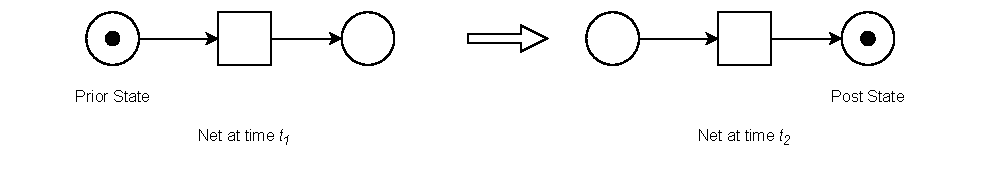
\includegraphics[width=\textwidth]{graphics/PN_Transduction.pdf}
\caption{\textbf{Transduction:
}The transducer is represented as a square node, which will fire when a condition of at least one token as input place value is satisfied, giving rise to the resulting place value.
Places are represented as circles with or without tokens (the values).}
\label{transduction} 
\end{figure}


A coordinated Pair (CP) generating FAPs
A coordinated Pair (CP) generating HAPs
How FAPs become HAPs



However, a pull action from the complement muscle between the cycle can generate a halting action in between.  Thus two actors can regulate each other's action without involving any other controlling agent or actor. If the pulling forces are equal and opposite, we may expect a jam, but variations in the pull may generate a resulting vector. A fine-grain halting may lead to greater coordination.  This is one model of implementing a simple haltable-action-pattern (HAP). \footnote{Citations to such explanatory models in kinesiology or mechanical engineering or robotics will be helpful.} 

There are two senses in which multiplicity plays an important role. One sense is similar FAPs at multiple locations (zones) of the organisms' body. The second is in the sense of variations among the zones based on action patterns.  For example, a biting action of the mouth differs from a waving action of the tail zone or a walking zone of limbs, while multiple walking zones exhibit similar patterns.  We use this sufficiently grounded assumption based on comparative anatomy of organisms to postulate the following \textit{dynamic principle of antagonism.}

Haltability, coordination of actions, emerges due to dynamic antagonism among the zones.  

\subsection{Body as a differentiated torus}
Most multi-cellular organisms during the development indicate that the underlying form is that of a torus. Specialized morphogenesis, leading to differentiation, the final shape appears differently. 

The broad body plan of a cognitive agent is tubular and topologically a torus. [Refer to wireframe diagram of C.Elegans]. A tubular architecture offers an inner as well as outer layer and the middle layer in between. The 3 components of concern for a cognitive architecture are (1) the sensory receptors organised as \textit{sensory boards (SB)}, (2) the motor action zones organised as \textit{motor boards (MB)} and (3) the connectors in between sensory and motor boards organised as a \textit{network}. Thus the body of a cognitive agent is modelled as a sensation modulating network (SMN). The nodes of the network include sensory and motor boards, while the edges include the connections of the network. Biologically, sensory boards are realised by sensory receptors, motor boards by the muscular and skeletal system and the edges of the network (connections) by the nervous system. It is important to keep in mind the contrasting point of the architecture with the received view that confines network only to the nervous systems, where the body of the neuron, the soma, forms the node, and the axons and dendrites form the connections.



The core proposal is to show that there exists a world within the body and a clear criterion of demarcation between the internal and external worlds. By doing this, we demonstrate that behavior is not restricted just between the body and the external world, but included action performed within the internal environment of the body. We demonstrate this possibility by modeling the body of a cognitive agent as \textit{a network situated in an environment} which includes other agents and physical systems. This is in contrast to the widely received view of a centralized computational brain controlling a sensory-motor body, which, in turn, interacts with the world out there.

The grounding of representations that we are attempting is achieved by remodelling the biological architecture (anatomy and physiology) of the body itself, in order to make internal environment possible.

\subsection{Biological Architecture for Cognition: Tubular, Polarised, Nested, Serial and Bilaterally Symmetrical Body Plan}

% \footnote{Contrast with brain-body-world schema} 
The broad body plan of the SMN is tubular and topologically a torus. [Refer to wireframe diagram of C.Elegans]. A tubular architecture offers an inner as well as outer layer and the middle layer in between. The 3 components of concern for a cognitive architecture are (1) the sensory receptors organised as \textit{sensory boards (SB)}, (2) the motor action zones organised as \textit{motor boards (MB)} and (3) the connectors in between sensory and motor boards organised as a \textit{network}. Thus the body of a cognitive agent is modelled as a sensation modulating network (SMN). The nodes of the network include sensory and motor boards, while the edges include the connections of the network. Biologically, sensory boards are realised by sensory receptors, motor boards by the muscular and skeletal system and the edges of the network (connections) by the nervous system. It is important to keep in mind the contrasting point of the architecture with the received view that confines network only to the nervous systems, where the body of the neuron, the soma, forms the node, and the axons and dendrites form the connections.

Sensory receptors are located in a distributed way across the body in the outer, inner and middle layers. The distribution of these nodes \textit{on} and \textit{in} the body is not uniform. Polarization exists, in the sense that some nodes are arranged densely on one-side of the tube. The sensory receptors are differentiated into specialised modalities transducing thermal, tactile, auditory, visual, olfactory, gustatory and location signals. The polarised and bilaterally symmetrical arrangement of these sensory receptors plays a significant role in constructing the picture of the internal and external world. The receptors organised as sensory boards are \textit{mounted} on the motor and mechanical boards (muscular and skeletal system). For example, a pair of eyes are located towards one pole of the body and absent at other places. Each eye has multiple photo-receptors and motor modulators, together constituting the nodes of the network. Similarly we see such concentrations of sensory receptors for other modalities. Although tactile receptors are located in a distributed way, their density varies from place to place on and in the body. This unequal distribution in location and density of sensory receptors plays an important role in differentiation and solving the problem of location. [Make a picture of praying mantis]. One more contrasting point of this model may be noted, that we consider the motor boards as sensory receptors of location, and not merely as actuators. As far as cognition is concerned, actuation is essentially for supporting sensation of every modality, committing to the theory of action based perception.

On this body plan, there are also multiple action zones. It is important to note that action zones are also oriented towards the inner layers of the tubular body plan of the agent. There are more action zones at the anterior side, particularly at the inner surface of the tube, making the body polarized. Animal anatomy describes this plan often in the name of cephalization, seen in almost all bilaterally symmetric beings. The significance of a polarized body plan and the existence of action zones at the inner surface becomes clear as we discuss the modulation mechanics below.

The schematic shown in figure~\ref{smn} shows a typical cognitive agent's polarized and bilaterally symmetric body plan, based on the model described here. Motor boards are present all over the body attached to the skeletal system that facilitates movement, while the sensory boards are mounted on moving structures at several action zones of the body. The term action zone is used in this article to refer to a complex of flexing areas, which are often located at an identifiable place in the body. For example, orbit of an eye, lip- movement, flexing the digits or toes, holding an object etc. [Based on the figure: We represented an assembly of motor boards as rectangular action zones at the interface of the body and the internal and external environment in the figure.]

Apart from the polarised distribution of sensory organs, it is important to note that the motor organs, which are also sense organs, are located in a \textit{nested} manner across the body.
A large set of highly specialized motor receptors (location sensors), are present across the body organized in a bilaterally symmetrical and hierarchical (nested) manner, which biologists call as skeletal or voluntary muscles. [Add a citation that supports the tree for skeletal and muscle anatomy.] In our model, insofar as cognition is concerned, skeletal muscles are sense organs, and their movement directly supports perception.  Biologically, muscles are considered as organs of movement and locomotion. In conventional cognitive science, their role is considered auxiliary. In our model, movement and locomotion are primarily cognitive functions. Apart from providing location data as a sensory subsystem, their \textit{characteristic} movement provides conceptual schemes employed in cognition. As this is a central and contrasting feature of the model, more elaboration on the characteristics of the movement are presented below.

The motor receptors of the network are unique, because they are mounted/embedded in a bundle of muscle fibres organised as \textit{boards}. This specialized plan is essential for playing the role of \textit{inferring} the location. The data from location sensors is created through movement. That is to say, the position is resolved only by change-in-position (displacement). But, location cannot be determined without data from the other sensory streams. We interpret location, like consciousness, as a dispositional concept. Location is always of some thing or the other, some sensation or the other, of some phenomena or the other. Employing a Kantian aphorism, we may say: location without sensory data is empty, and sensory data without location is blind. Moreover, it is not only that location cannot be calculated without movement, the construction of an image of the world through other senses is impossible without spatio-temporal data. Action is essential for resolving both space and time. What makes an action possible, is a foundation question, but it is beyond the focus of this paper.

\emph{Elaborate on synchronicity and serial aspect of the actions to resolve time.}

The source of temporal data is the serial action pattern.The body plan is not only polarised and nested, but also serial in nature. We also assume availability of repeatable actions, beats within the body, providing a temporal canvas/ stage. The availability of the temporal stage/ canvas is granted by the existence of metabolic cycles, biological clocks is well established [cite] in terms of diurnal and biurnal rhythms.\footnote{need to elaborate with right vocabulary and cite relevant sources}.


Antagonistic action is a key character of the body plan, which plays an important role in the current model. 

The body is not a complete network.\footnote{In graph theory, a complete network is defined as a graph where each node is connected to every other node.} Some SMNs are connected to only certain others. The model uses the principle: ``Fire together. Wire together'' (FTWT) \cite{hebb1949organisation}\emph{Principle: Fire Together Wire Together}. The SMNs that are recurrently active at the same time are likely to get connected over a period of time. Thus the connection `board' is plastic, not static. The connection patterns are created, reinforced and modified based on the dynamics of the body (action patterns) in its ontogeny (developmental history). The implication of the FTWT principle is that the actions determine the connections, and not the other way around. However, much of the differential connections may have been already determined by phylogenetic and prenatal action history. Though it appears as though the agent starts with an undifferentiated state, the phylogenetic and prenatal action history bestows, practically, a body with `innate' action schemas at birth.\emph{Affinity with Nativism} In a model where actions are located at the interface between the body and the environment, the actions within the body (including the prenatal stage) are often ignored (e.g. suckling, swallowing action-patterns etc.). In our model, the most stable and determining action schemas are already in place by the time the agent is exposed to the external environment after birth.

The array of receptors as a board are connected by an incoming bundle of sensory neurons to the DFN as shown in the figure.


We shall discuss the origin of differential connections and various possibilities of their implementation in the section~\ref{mbr}.

In the schematic shown in figure~\ref{smn} the connections within the IN are not drawn to avoid clutter. The arrows between action zones (Z-A to Z-H) represent modulation of the zones, and not the connections. 

\begin{figure}[ht] 
%\renewcommand{\thefigure}{2}
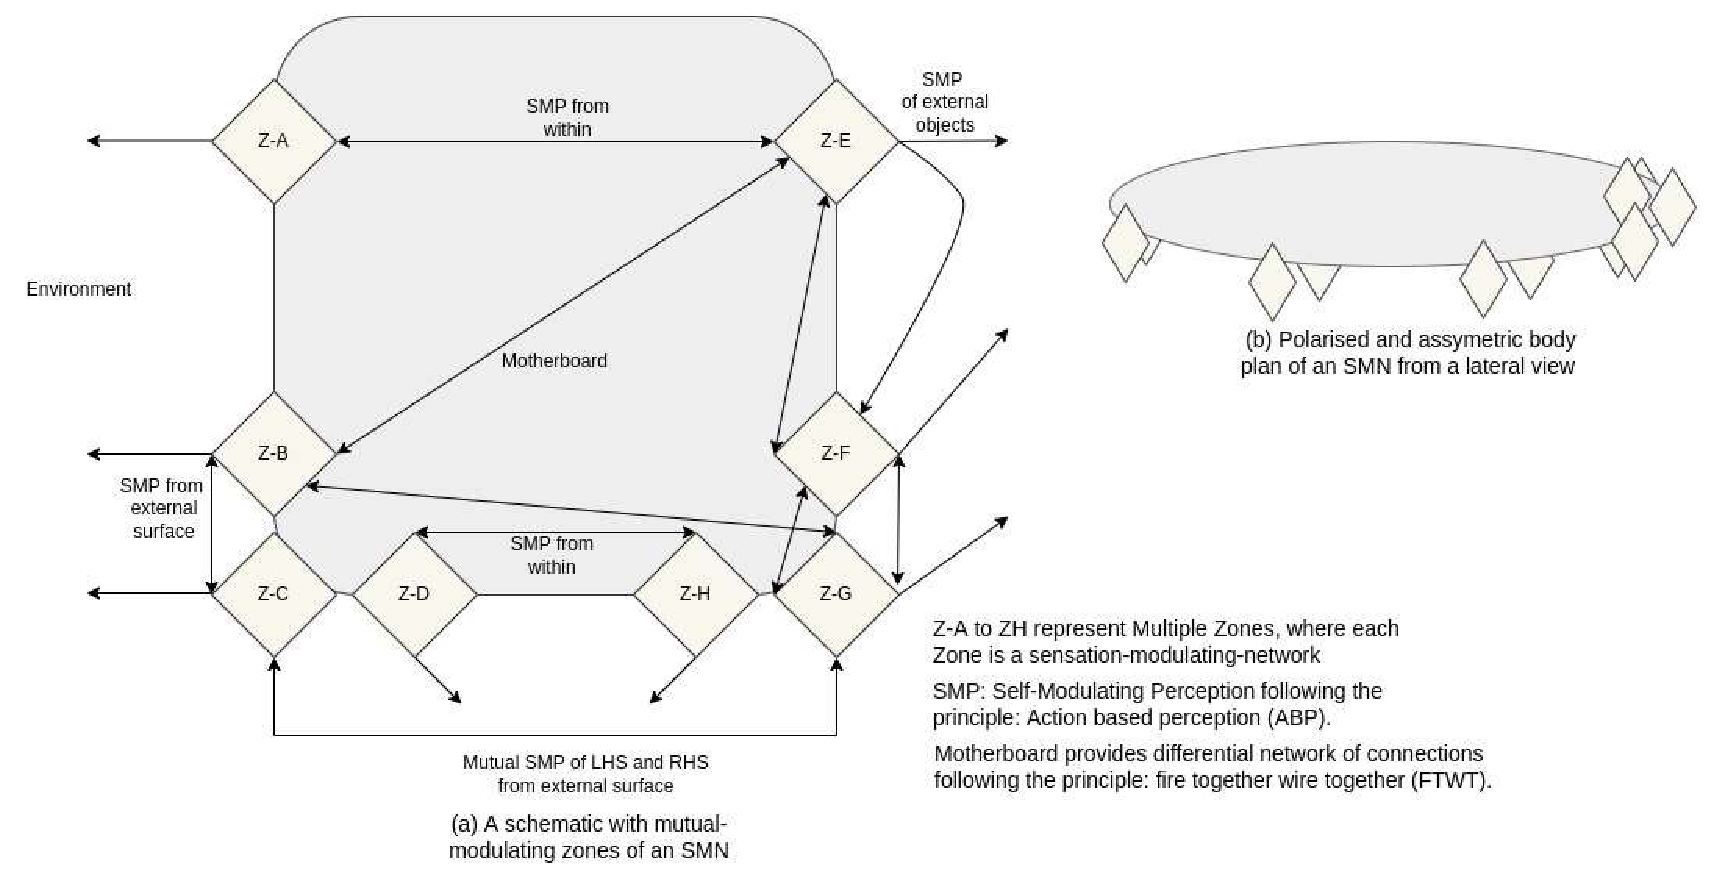
\includegraphics[width=\textwidth]{self-modulating-perception.pdf}
\caption{\color{Gray} \textbf{A schematic representing a cognitive agent as a network of multiple self-modulatable zones.}}
\label{smn} % \label works only AFTER \caption within figure environment
\end{figure}

The outgoing arrows from the zones represent the sensory modulation from an external world invoking action based perception (ABP) \cite{noe_action_2004}\emph{Principle: Action-based Perception}. According to this principle, the perception is not a passive sensing of the world out there, but an active process.

The same principle is employed when an action zone modulates another action zone within the body. This implies that ABP is used for perceiving both the worlds (internal and external). The double headed arrows in the figure represent mutually modulating zones. Between Z-B and Z-C, the double-headed arrow represents mutual modulation from the outer surface. For example, consider a fidgeting action between fingers touching side-ways, the hand touching the chin in the typical thinking posture, scratching an itch on the same side of the body etc. The double-headed arrow between Z-C and Z-G represents another mutual modulation from an outer surface (e.g. clapping with hands), LHS and RHS mutually modulating.
In a well-connected body, the implementation of a single-headed arrow between two zones (like Z-E and Z-F) appears very rare. However, to understand such a possibility, we can consider touching a numb leg, where due to temporary lack of internal feedback, mutual modulation is transiently unavailable.

The double-headed arrow between Z-D and Z-H could represent mutual modulation between the action zones from within the body. For example, swallowing zone and speech zone. In the case of swallowing, with or without food, the upper and lower surfaces of the buccal cavity, pharyngeal zones mutually touch and modulate each other.

\emph{Principle: Body-plan as torus.} But it is very important to realise that this internal and external distinction would vanish when we bring to our attention the topological architecture of the body, which is a torus. Therefore, the apparently internal surface of the body is topologically external. 

Mutual modulation of action within the body is an important and contrasting feature of the model, which is largely ignored in the current discussions in cognitive science.\label{contrast-internal-ABP}\emph{Principle: Self-modulation.} This mutual modulation, within the body, is a core cognitive mechanism in the current model, which appears very early on during the prenatal stage itself. Therefore, we locate the roots of cognition within mutual modulation within the body (internal environment). 

Often, self modulating actions, such as thinking, are considered as recent evolutionary features, whereas in our model, the very root of cognition is due to such internal mutual modulation, though it is counter-intuitive. The world within the body is missed in the current accounts. Since this is a contrasting feature, more elaboration on this follows in the model.


We described the body as a network of sensory and motor boards. We provided an indication of how the body acts on itself and with other things in the world.  We will now turn to describe the details of sensory modulation. 

\begin{figure}[ht] 
%\renewcommand{\thefigure}{2}
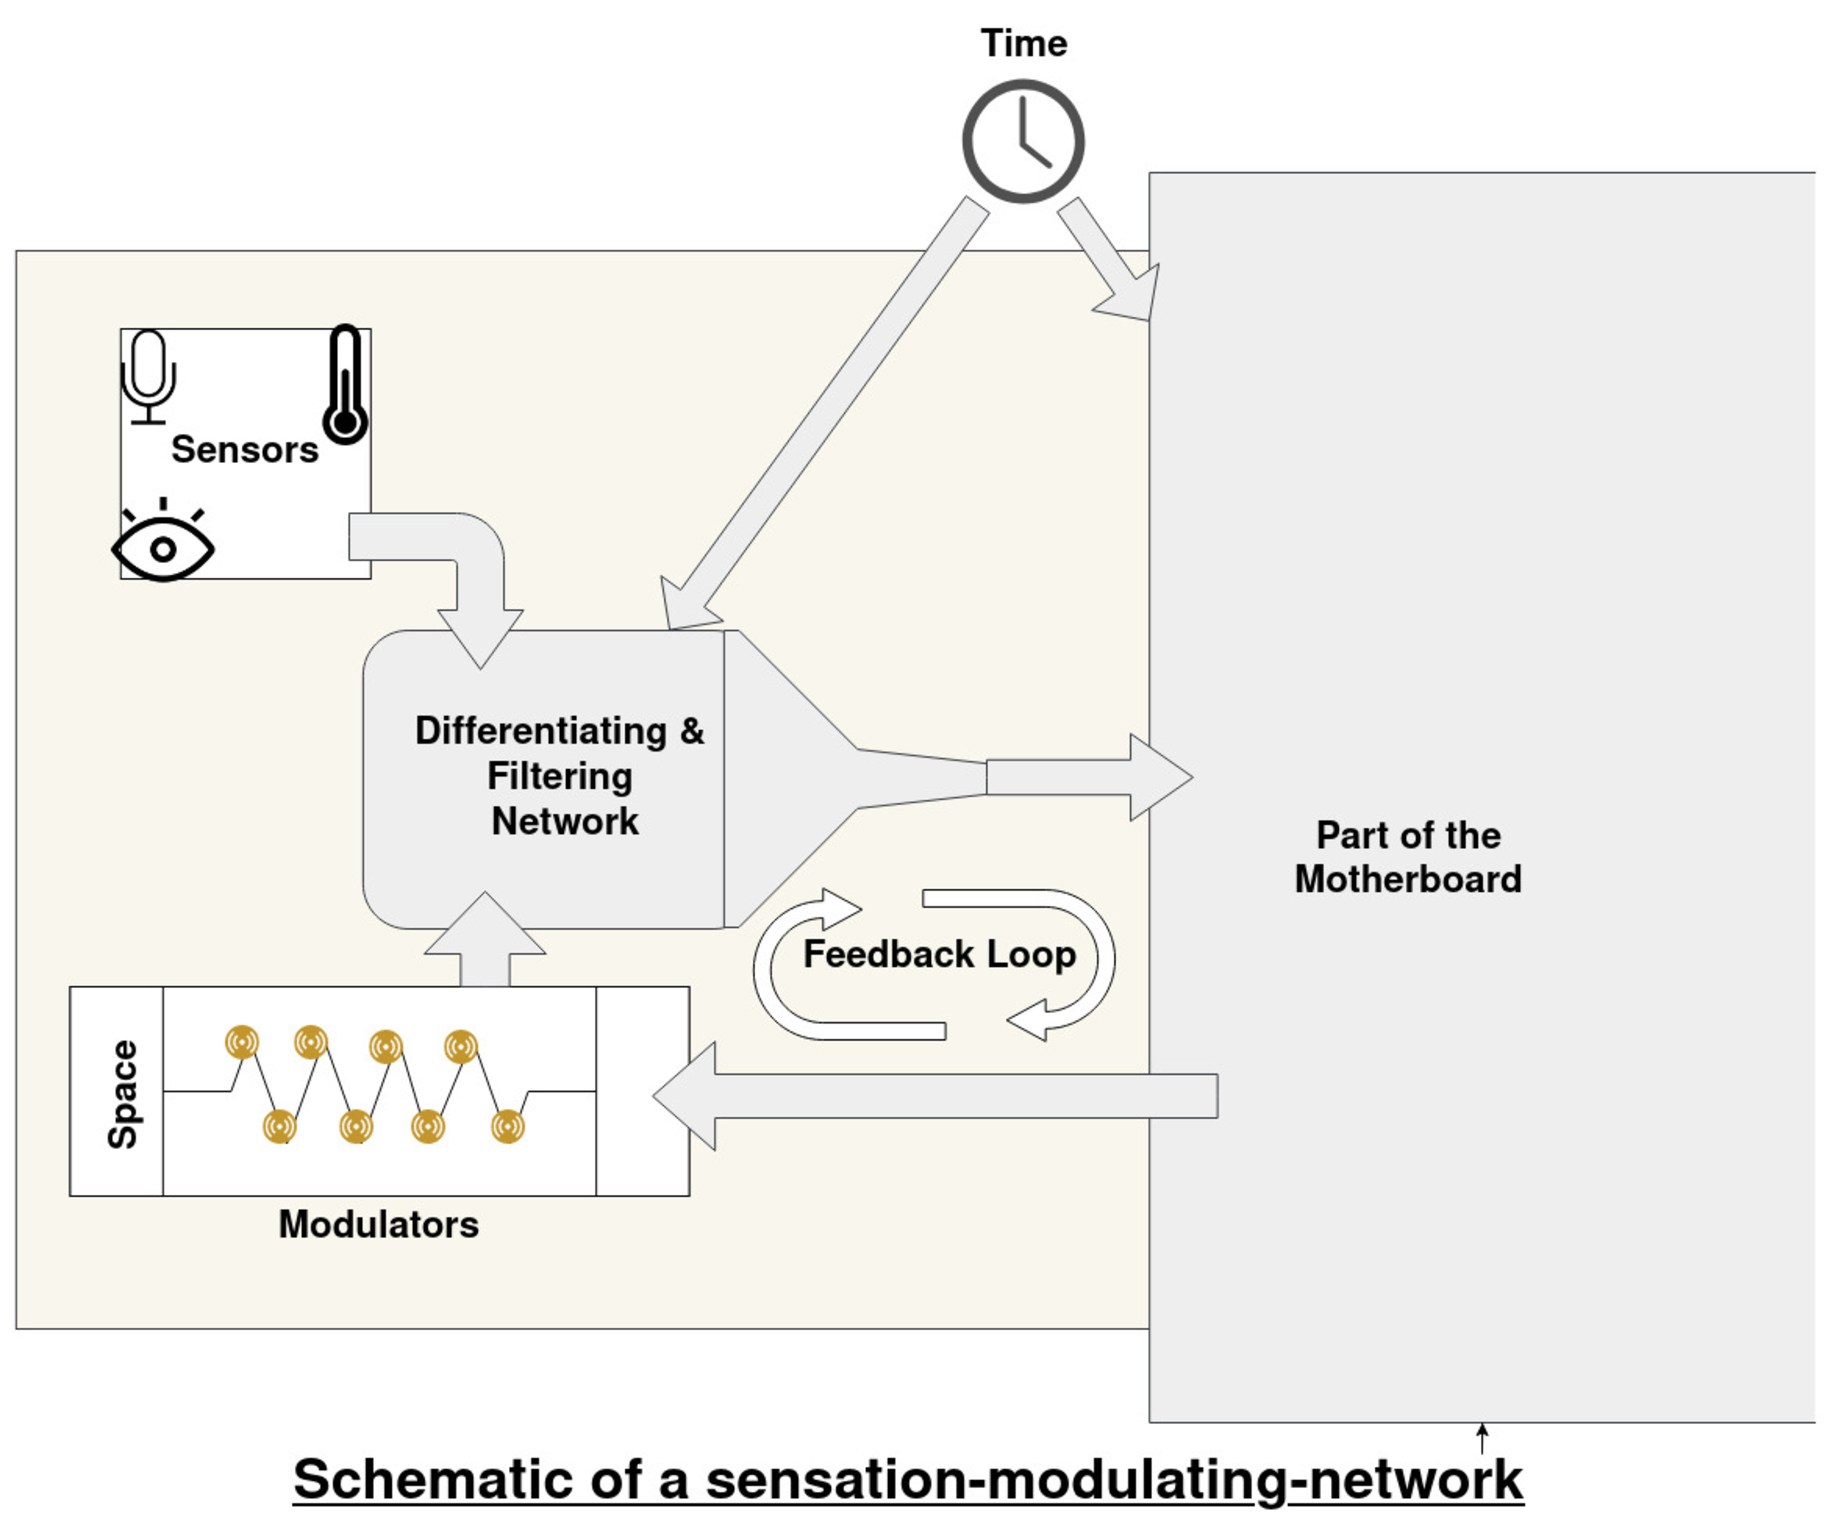
\includegraphics[width=\textwidth]{structure-of-Zone.pdf}
\caption{\color{Gray} \textbf{A schematic of a perception modulating action zone.}}
\label{zone} % \label works only AFTER \caption within figure environment
\end{figure}

\subsection{A Network of Sensation modulating networks}

\subsubsection{}

The structure of a cognitive agent's body is modeled as a nested network of Sensation Modulating Networks $\{n(SMN)\}$. And the dynamics of cognition is modeled as differentiation of Differences $\{\delta(D)\}$ in a  multi-modal sensory stream.

It is important to underline, as a point of contrast, that the Central Nervous System (CNS) is not interpreted as \textit{the} network in our model, but a part of it. The entire cognitive agent's body is a network. CNS provides only the differential connections between different DFNs and among the nodes (sensory and motor receptors). Therefore the popular schema of brain-body-world is reduced to body-world. Since the body is a network of SMN, this schema can be represented as 
\begin{equation}
[\{n(SMN)\}\rightleftharpoons \{W_I\}] \rightleftharpoons \{W_E\},
\end{equation}

where $W_I$ is the internal world and $W_E$ is the external world.  $W_I$ can be substituted with another $\{n(SMN)\}$, since it is nothing but another $W_I$ in effect. 


Thus the above representation can be re-written as 
\begin{equation}
[\{n(SMN)\}_i\rightleftharpoons \{n(SMN)\}_j]\rightleftharpoons \{W_E\}.
\end{equation}
What constitutes the internal world will become clear once we make the principle of mutual modulation clear below.


This schema can be contrasted with the brain-body-world schema, which can be represented as 

\begin{equation}
\{CNS\}\rightleftharpoons\{B\}\rightleftharpoons\{W_E\}
\end{equation}

where the CNS is the central nervous system, B is the rest of body and $W_E$ is the external world.

Consider the functional network as a $\Delta$ network of a set of sensory boards $\{S_i\}$ and motor boards $\{M_j\}$. We represent this network as \begin{equation}\label{delta_notation}\Delta^{\{S_i\}}_{\{M_j\}}, or simply, as  \Delta^{\{i\}}_{\{j\}},\end{equation} where the subscripts always refer to motor boards, and superscripts to the sensory boards. For example, if $S_1$, $S_2$, $S_4$ and $M_1$, $M_5$, constitute a transient network at any given time $t_1$, this state of the SMN can be represented as 
\begin{equation}\label{delta_eg}SMN(t_1) = \Delta^{1,2,4}_{1,5}\end{equation} This $\Delta$ network is an ephemeral functional state corresponding to a particular action performed by the cognitive agent at $t_1$. Thus differentiation of Differences is realised in $\Delta$ networks, where the motor boards differentiate on the Differences streaming from the multi-modal sensory boards. This is how we resolve every action as a functional network of sensory motor subsystems.

Differences are given and taken from the environment directly, while differentiation is an active function of the agent. This active function can resolve modalities and selectively attend to a difference in the stream.

SMNs are functional states of the cognitive agent. This identifiable functional state does differentiation and filtering. Since each SMN is a network, the body is a network of networks. We may represent the active cognitive agent as $\{n(SMN)\}$. The first order network of SMN is a functional sub-graph. By functional subgraph, we mean, it is not distinguished based on structure, but by ephemeral or transient connections. SMN is hence localizable, but ephemerally.

An analogy with modern communication infrastructure helps here. When a group of people are present in a global online meeting, the people are connected through their devices. The people and their devices are localized in space, but available to other locations at about the same time. A bunch of ISPs (Internet Service Providers) enable these connections through networking boards called routers. Though the networking routers of each of the ISPs are distributed geographically, the location of the networking router is not relevant, as long as the router is accessible to the devices. Some of them may be connected through mobile networking access points, while others are connected through copper wire, and yet some others through optical fibre. How they are connected is not relevant, as long as they are connected somehow.

In a cognitive agent's body, the location of sense organs may be distributed anywhere in the body. The stream of signals coming from them at a given time is part of the \textit{cognitive engagement} only when the sense organs are modulated. Though the existence of neurons (wiring) determines connections, the actual connection gets established when the wires actually get fired at the right time. What visual or auditory stream is available at a given time is determined by what actions are carried out at the time. The sight and sound stream, e.g., should be tuned to a situated action.
Considering the actions such as talking, walking, turning etc. as determiners of active connections at a given time, we consider an SMN as a dynamically actualized region of the possible networks the body plan offers. Just as the subscribers of an online meeting are registered by seeking to be part of the meeting, in a cognitive engagement only a set of the stream of sensations are considered a part of it, while the rest are ignored. We shall elaborate this mechanism below.

Let us be warned that the analogy with an online meeting is employed only to bring home the point that the SMN is a dynamic network actualized among the possible configurations of the body plan. Just as the connections established for a specific online meeting is one of the several possibilities the Internet offers, the SMN is a dynamically actualized network formed transiently among the various possibilities the network provides. The network is not a localized structure, though the nodes of the network (motor and sensory boards) are. As we proceed further, we shall take more examples to gain clarifications on the structure and dynamics of SMN, which may differ from the online meeting analogy used here.

When an SMN is described in terms of its function, we can expand the acronym as sensation modulating network. In terms of the structure a cognitive agent's body can be described as sensory motor network. The expansion of acronyms can therefore be contextual. For example, the functional network is of $\Delta$s, and the structural network is of the sensory motor boards.

Each sensory board is an array of localised sensory receptors (transducers), which connect through a bundle of connectors (a bus) to a differentiating and filtering network (DFN). Each motor board is an array of location-receptors mounted on a bundle of actuators (muscle-fibers). The motor board connects through a bundle of connectors to the DFN on the one hand, and receives connections from the integrating network (IN) on the other. The DFN and IN are distinguishable only on the basis of their function and the nature of connections, and need not be localized in any specific area of the central nervous system (CNS).

The motor board can be considered as a mediating board between a DFN and IN. In other words, the motor board is sandwiched between the DFN and IN, creating dynamic and transient loops. Speaking of the network in graph-theoretic terms, we can say that, the nodes of an SMN are arrays of receptors and actuators, and the edges are dynamically distributed bundles of connections manifesting the aforementioned loop.
Though the network appears bilaterally symmetrical, the SMN extends both sides. The connections can be distinguished into those that come from the receptors (sensory as well as location sensors in motor boards) to the DFN, and those that come from the IN to the actuators.




\subsection{Sensation Modulating Network}
Let us recall that the units of modulation, namely SMN, may be located in a distributed manner, and therefore the boundaries of SMN are identified and defined only on the basis of how the components of a unit are connected to each other, and not on the basis of their location. Therefore, to be considered part of an SMN, the components can be anywhere in the body. The boundaries of zones are defined only functionally, not anatomically. It is identifiable only as a dynamic sub-graph of a network, thus making the network ephemeral. The figure~\ref{zone} describes the sensation modulating network.

The difference between mounting and being connected may be clarified through a thought experiment. Sense organs have to be mounted on a moving part of a body, or a moving body. This is necessary for sensory modulation. In the absence of sensory modulation, the information stream passing through the sense organs remains unprocessed.

The sensory (transducers) boards are specialised for a specific modality, such as light (visual), sound (auditory), smell (olfactory), taste (gustatory), touch (tactile) and location (spatio-temporal). The motor boards are modulators (actuators) and are transducers for location data. The clock at the top indicates the availability of time to the system. Thus time, location and other sensory modalities are available to the differentiating and filtering network (DFN). DFN connects to other SMNs through the IN. {The connection between locating, addressing, attention, naming, retrieval, re-moving, memory, recollection, etc. needs to be elaborated at an appropriate place.}

The stream of sensations/signals, which is a result of transduction, enters this network undifferentiated. What is transduced is determined by the limits of the transducers, which developed evolutionarily. There are biochemical activities that keep the transducers charged and refreshed. Though it is passive from a cognitive point of view, it is not passive from a biological point of view. 

For example, the transducers (rods and cones) in the retina have to be in a polarised state prior to light falling on them. The light perturbs and depolarizes them, which generates a stream of signals. The refreshing process of repolarization is a process of compensation/repairing/restoration. During this period of restoration, the transducers are incapable of generating any signal, even if environmental inputs are present. This layer of activity is metabolic and does expend energy for its maintenance to keep the zone active. The mechanism at this layer generates \textit{differences}, but no differentiation takes place. 

An implication of this for cognition in our model is that it is not available for conscious cognition, though the adaptive biological aspects of life are available. The adapted environment where the organisms could live/sustain depends on the availability of the refreshing metabolic process. When such a process is not available, the sensory differences required for cognition are also not available. Though the organism spends energy for the refreshing process, this is affordable to the organism. If the process of sensation itself is more expensive than the basic survival mechanisms, the variations would not have evolved through natural selection. This means that another layer of metabolic activity exists that makes the sensory mechanism available. The frequency of refreshing cycles at this physiological layer must be higher than the refreshing cycles of the sensory layer. Unless the deeper layers generate a sufficient surplus, the upper layers may not remain in an active state. An implication of this layered ontology is that the conscious cognition depends on the surplus made available by the core metabolic layers.

The range of sensations that are possible for an organism depends on the refresh/repair mechanisms available to it. For example, the spectrum of sound or light, or the extent of touch that the organism can differentiate, must fall within the economic zone of refresh/repair mechanisms. When the organism is exposed to extreme ends of the spectrum, there exists a potential danger for survival, since the repair mechanisms don't exist. \footnote{Apart from survival, the aspect of aging/functional changes – both positive and negative – can be explicated.}

The above elaboration portrays the dependency relation between the physiological and sensory layers. We now turn to the next point of dependency relation between the sensory/transducer layer and the motor/actuator layer. Thus we move from differences to differentiation. 

When actuators move, there is a corresponding change in the input stream. The action \textit{interrupts} the stream. Whatever sensory stream that enters at the time of action becomes phenomena. The entire stream does not constitute percept, but only that which is acted upon. Thus this process is active, not passive. One effect of this action is filtering. \emph{The world may have a rich structure but it is not accessible to the agent until acted upon through cognitive exploration. Move it to another appropriate place in the article.}

Apart from filtering, actions can also resolve the structure in the phenomena because the actions may not be monotonous, they may have a pattern. The changes in pattern can resolve details available in the phenomena. The change in pattern can be in terms of temporal characteristics like pause, frequency or speed. Grasping the structure in the phenomena corresponds directly to the action patterns. The poorer the action patterns, the poorer the structure of the phenomena will be. Though the structure of the phenomena is constructed, it cannot be generated without a corresponding structure in the world. 

In a cognitive model, not using ABP, richer action patterns in an empty external world should not produce a phenomenon. However, in our model, actions always generate phenomena, because every action perturbs the internal world. Thus differentiation due to action works only when the objects \textit{out/in} there can be differentiated. Absent variations cannot be generated purely out of richer action patterns.  But, without actions there are no phenomena. We shall see later (a) how we may explain what we perceive in a dream (b) how the criteria between \textit{out} there and \textit{in} there can be differentiated. 

Another vital role of the actuators is to differentiate the incoming stream of signals into different modalities. The changes in the sensory stream at the time of action, can be obtained by differentially and recurrently modulating the sensory stream.
For example, moving the head sideways, or moving the eye ball in different directions, moving close to/ away from the source of sound, closing eyes/ears etc., impacts changes in the sensory stream. The change in the visual stream, at the time when the head or the body moves, is differentiated from the change in other modalities. The apparent independent changes in the stream of any sensory modality while moving are differentiated just on the basis of the corresponding rate of change. Holding some aspect constant, while changing another aspect, is modulation. An analogy of this model with the nature of experimentation will be discussed further in the next section.

Thus, modulation does two more things apart from filtering (attention). One, it helps in differentiating the signals into different modalities. Two, it helps in calculating the rate at which each of the modalities are changing in a given stream. All the three operations, filtering, separating modalities, and correlating with the rate of change, are part of an active cognitive processing, which can be called \textit{differentiation of the differences}\emph{Cognition is differentiating the differences}.

The active processing done in cognition happens in the DFN. The filtering process economises the amount of processing required for cognition. The result of this is a richer set of a stream of differentiated data about the environment, which passes onto the IN.

The DFN does the filtering and differentiation due to the motor boards available all over the body, modulating the sensations. We are only ascribing a descriptive role to the DFN, without explicating the detailed mechanism describing exactly how it happens. However, the speculation is grounded, because we know from electronics that networks are capable of computation, depending on the differential nature of logical connections.  We propose that the data is constructed by the DFN by involving the mediating and modulating motor boards as nodes of the network. What happens in DFN is active while what happens in IN is passive. Passive doesn't mean insignificant, but no further processing is required. What happens from the IN is a composite self, a very significant emergent outcome. 

Often the current models recognise only touch, vision, gustatory, auditory, olfactory and proprioceptic sensations. Thus, the modulatory part of the body, such as muscles, provide only proprioception. However in our model, we consider actuators as fundamental sense organs providing spatio-temporal information not only from within the body, but also locating the body in the space-time with respect to the rest of the external environment by providing space and time information. We shall elaborate exactly how this demarcation of internal and external environments happens in the next section.

We make an assumption that the location information (position) is sensed not by direct observation, but through displacement (a measure of change of position). Given this assumption, if there are no action generating actuators, and if there exists no differentiable sensory stream the position sensors on them generate no useful information.

Why computing location is such an important process of cognition? Our argument is based on the assumption that atemporal pattern, such as a picture, is a constellation.  In a constellation the spatial relations between various elements are held constant. A recognition of a pattern depends on recognizing the constellation of relations, which are invariant.  E.g., face recognition. The various pieces of the face and their positions can be arranged logically in various ways. Unless the pieces are placed relative each other in a correct way, we cannot coherently regenerate the face. Keeping the pieces of the face constant, if we change the spacial relations between them, we can generate different faces. This geometrical transformation applies not only in understanding faces, but also the evolution of variations of forms in the living world.\cite{thompson1942growth} It is through a calculus of dynamic transformations we grasp geometrical patterns in the world.

As stated already, there are multiple SMNs in the cognitive agent's body, which is modeled as a network of SMNs. All the SMNs are connected through the IN, which provides an integrating and differentiating experience depending on the nature of connections. The analysis of experience happens at the SMNs, while the interconnections in IN provide the synthesis. As mentioned earlier what happens in IN is passive, while what happens in DFN is active. Maintenance of polarity of wiring of the network does need a lot of activity, but this activity happens at a core metabolic layer of the body. The networks are power hungry, since each firing of signal discharges the wires. It is assumed in this model that maintaining the potential by repolarizing or refreshing them happens by the metabolic activities of the biological layer. Cognitive layer depends on the biological layer.  We shall see in the later section that this separation of cognitive actions from biological actions happens through affordable disengagement.

{\emph{ Write Summary of the model section}


\section{The Functional Model of the Cognitive Agent}


In this section we present an argument that the human cognitive life, for that matter of any other cognitive agent, cannot be explained without an asymmetrical ontology and a gap-creating epistemology.  

\emph{The asymmetry condition is satisfied by polarized body plan and a bilaterally symmetrical localization of sensory and motor boards.} The asymmetry condition is satisfied by polarized body plan and a bilaterally symmetrical localization of sensory and motor boards. 
The structural body plan provides an embodied action schema for grasping the world. It is more natural for most of the animals to walk, run, swim or fly forward than backward because of the body plan. The architecture of the limbs of all the terrestrial organisms is asymmetrical, based on a limited degrees of freedom at each joint. Polarized orientation of the body to the ground with ventral and dorsal body differentiated, facilitates dealing with the field of gravitation. For example, an organism with sphere like body with feet all around can not differentiate the orientations (front-back, side-ways, up-down). All movement must deal with the given field, which itself is polarized. Legs in such a field cannot move, if the body plan is not antagonistic to the field. The anatomy of aquatic creatures also have to deal with the gravitational field, but it is not as pronounced as it is with terrestrial beings due to other aquatic forces. Anterior to posterior polarization is more pronounced in aquatic beings than dorsal and ventral. Since animal locomotion is an attempt to resist or oppose it's inertial state of motion, the architecture of the body plan must support it by allowing it to apply force. The asymmetry manifested in the arrangement of bones in the feet of any animal enables the organism to exert this force thereby constructing the orientation (front-back) with respect to the body and in relation to the environment. A symmetrical body plan can not provide a frame of reference.

The bilateral symmetry facilitates in alternating action patterns (e.g. movements alternating in legs while walking, running etc.) and a possibility of antagonistic action patterns. The antagonism in the body plan is so intrinsic that every joint functions through opposing pairs of muscles. This is possibly the only way how the inertia can be resisted, because one needs to apply force only for contraction. Since contraction is the only way of getting work done antagonism in the anatomical design is the only way to balance.\emph{Embodied experimental design as a cognitive foundation} Concentration of sensory boards in association with opposing motor architecture facilitates modulation. This concentration is a requirement for the experimental analysis of the world, since the environment impacts the body in a diffused way. The diffused environment requires a concentrated action to resolve the impact. Just as the experimental design in a scientific lab provides a means of regulating one variable while allowing the impact of another, the body architecture of animals is that of a living laboratory. The engineering design employed in scientific experiments is an extended body plan.

\emph{A formatted body and its action patterns determines the structure of the phenomena.} Specialized sensory boards are also organized to suit this body plan. As a result, the possible action schemes can resolve the structure of the world. This resolution is logically impossible without movement, and most importantly the patterns of movement facilitated by the body plan. The problems of cognition cannot be resolved without addressing this basal mechanism. Mere sense organs and the nervous system are not sufficient to build a complete framework. The nervous system cannot process the data stream coming from sensory organs without a mediating and modulatory system. Data can be stored only if we have a formatted body. The format of the body is not only the structure, but also the format of actions. The action patterns depend on the body, modeled as a sensory-motor network.  We shall elaborate on how this model could ground cognition in this section.

\emph{Framing problem} A stream of uninterrupted sensations may have a pattern, and it can be processed to identify the pattern. Here we are assuming that the existence of a pattern and its identification is the essence of information processing. It can be done by our modern computers, which are capable of recognizing patterns and establishing correlations as well. But this is an ungrounded process, because, \textit{on its own} the machine cannot detect: Where does the stream come from, from within the machine or outside? Which pattern to attend to? Which pattern is more significant than the other? Which ones to ignore? This is the framing problem. This problem is related to how a cognitive agent understands the context/situation.

Recognition of patterns and relating the patterns to a context is not sufficient for grounding semiotics. We now turn our attention to the formulation and resolution of naming-framing problem.

\emph{Naming problem} Apart from the understanding of context, we need to deal with naming and referencing. Information processing is not only impossible without names but also useless if it cannot name the patterns. One may program the machine to give distinct names to distinct patterns, and can also group them nicely based on some similarity detecting algorithms. It may also develop a complex ontology at the end. But how does the machine establish a reference, of which patterns pertains to which object in the world, or within the machine? And more importantly how could it convey to us the \textit{private} naming convention?  Can the machine at least tell them to itself?  If so how? These are three philosophical problems at one go: concept formation, symbol grounding problem and that of possibility or impossibility of a private language. Variation in the world and a capacity to detect patterns in a stream of experience is not sufficient to give names to the patterns. We need a naming mechanism in a cognitive agent, and we need a mechanism to communicate with each other, in a community of agents, through names. Let's call this \textit{the naming problem.} 

Combining the above two problems, let us call them together a \textit{naming-framing problem}, because we think that the frame problem and symbol grounding problem are intrinsically related.
We will now argue that the naming-framing problem can be solved through modulation. In other words, referencing and distinguishing the external world from the internal world will be shown to be possible through the same mechanism.

A world that is homogeneous is no world at all. It offers nothing to know. There are no affordances to offer. Nothing to act on or interact with. For the argument's sake, if we place a cognitive agent in such a homogeneous world, it will not even know if there is a stream at all in her experience, forget about detecting or identifying patterns in them. So, we assume that the world is heterogeneous.   

Let's place a community of cognitive agents, with the structure and dynamics specified in the $\{n(SMN)\}$ model presented above, in a heterogeneous world. We shall now present how such an agent can make sense of the world, and what else we need to develop language and culture. As mentioned in the introduction, the framework that is proposed here is based on an ontology of actions, and not interactions. The model of a cognitive agent presented in the above section describes the body as a network of modulators. A modulator in the scheme is the location of the action. We will now account for gaps in actions, and their role in the naming-framing problem.

What is needed in such a modulating unit in order to do its job, namely to regulate, to modulate? For argument's sake, suppose there is an action that happens relentlessly at an invariable frequency, what kind of differentiation can we expect from such an actuator? However, such relentlessly recurring actions are commonly found among animals. Even in higher animals like humans, beating patterns like heartbeat are uninterruptible. There could be a range of variations in the frequency and amplitude of these beats, which can be modulated by modifying physiological conditions. But such beats, when halted/ paused, may prove fatal to the organism. Halting such action patterns is physiologically unaffordable.

Let us recollect the architectural plan of the body. First, the modulators are distributed across the body in a polarised and bilaterally symmetrical manner. They are concentrated more to one side than the other. This body plan is to defy the forces, flows and fields in the world whenever and wherever possible. Yielding or total submission to the external environment cannot generate knowledge about the environment. Developing this ability to resist is \textit{action}. When we say the model is \textit{enactive}, it implies this condition.

\marginnote{The principle of layering} Since modulating certain beats such as heartbeats is not affordable, we may consider situating actions over and above the core physiological mechanisms. In order for the actions to be affordable, the interactions of the sustaining layer  must continue, and they should generate sufficient surplus. When we say cognition is enactive, it implies that the emancipation from sustaining mechanisms is expensive. Though autopoietic mechanisms may include actions, they are uninterruptible, hence no liberty to introduce gaps here. Hence autopoiesis as a mechanism to compensate the lost energy and matter takes care of the sustaining layer and provides the necessary surplus in the system making actions possible \cite{maturana1991autopoiesis}. This is also an action, but the uninterrupted pace at which this action takes place has no liberty for introducing \textit{gaps} in this layer. In other words, the system can't physiologically afford to halt. However, it is this state that could enable ephemeral actions on the periphery of an autopoietic system whenever and wherever possible. This is made possible by a differentiated body plan that enables a division of labour. Some layers are busy in not only replenishing the loss of energy and matter but also generating surplus energy and matter, such that other layers in the body can \textit{halt}. This design now has room for free action. In this perspective, it is an uninterrupted action of some layer that grants freedom to some other layers. It is this partial break from uninterrupted work, that gives rise to the freedom to enter into the cognitive domain. It is in this subtle sense, that our model differs from Maturana and Varela's account of the connections between biology and cognition. The subtlety we introduce is haltability. 

This differentiation of layers, as against the uniform distribution of work, in a system facilitating deviation from the normal course of actions, gave rise to the roots of cognitive state. We shall call this \textit{the principle of layering}, which is over and above the design principles of polarization and asymmetry we discussed earlier. The sense of being over and above can be characterised by naming metaphorically, this principle as epi-physiological or epi-biological.

\emph{Biological roots of disengagement} Beats, as uninterrupted action patterns, support the agents to move. If an entire body is engaged in movement, as in the case of some worms, the degrees of freedom are limited. In an earthworm, the ingestion beats and locomotion beats are coupled. The worm cannot move (locomotion) without eating (when in a burrowing habitat --- soil), and cannot eat without locomotion. In another body plan, say of nematodes, the ingestion movement in the buccal zone is independent of the locomotion. This sort of decoupling of functions emancipates one zone from the other. The worm can feed without moving the entire body, and move without feeding.

\emph{Homologous roots of anatomical disengagement, modulation and haltability} These examples indicate how one could speculatively weave a story of the evolution as a story of decoupling the body into multiple zones, where each zone can act partially independent from another, and exhibit a distinguishable action pattern. The development of tongue, lips, jaws, pharynx, larynx, gills, lungs, fins, tails, ears, eyes, limbs, toes, fingers, neck, shoulder, hip and so on are interpreted in this story as anatomical disengagement (or decoupling). One can draw a tree of anatomical disengagement representing the epi-physiological bifurcation over and above the phylogenetic tree of evolution. For example, in early vertebrates as in cephalopods, the feeding and breathing action patterns (filter feeding habit) are not decoupled. In Gnathostoms, we see the stoma (mouth) differentiated through the evolution of jaws enabling decoupled breathing habits from feeding habits. Episodes of decoupling could be reconstructed for the evolution of simpler buccal cavity differentiated into complex cavity, developing teeth, tongue, lips, pharynx, larynx etc. In parallel, an undulating body (as in lampreys) gets decoupled into localised and bilaterally symmetrical fins, decoupling locomotion as a entire-body function. Similarly, one could consider the decoupling of the undulating alimentary canal from the entire undulation of the body. These episodes of differentiation might have been naturally selected because of the economic value of decoupling, as localised movement is inexpensive than whole body movement. Each episode of such differentiation is an episode of decoupling leading to the evolution of independent action patterns (habits). Thus the gradual polarisation and bilateral symmetry of the body-plan through evolution leading to differentiation of action zones can be woven into a phylogenetic story of decoupled and localised zones of action patterns (habits).

Lets call the tightly-coupled actions as \textit{harder-actions} (e.g. the coupling between locomotion and feeding in the earthworms), and the decoupled actions as \textit{softer-actions} \cite{nagarjuna_muscularity_2005}. During the course of evolution more anatomical disengagements may have given rise to the availability of more such softer-actions.

We need to cut the story short to revert back to how the transformation of a tightly coupled body plan into a loosely-coupled body plan, from harder-actions to softer-actions, is relevant as a context for cognitive science. The cognitive hypothesis we propose, given this transformation of the body plan, is: the greater the disengagement of differentiated action zones, the greater is the agent's capacity to modulate the incoming stream of experiences. This disengagement itself is a function of anatomical polarization and layering.

This disengagement has an economic dimension, without which it is difficult to understand how it could have played a role in natural selection. The agent can do more work with less effort (spending less energy) because of disengagement. A body plan of an organism that has a coupled movement for both ingestion and locomotion is expensive, than when they are decoupled. Moving when not eating, or eating when not moving is a new found possibility.

Once we have multiple softer-action zones, it is possible to rest some while the others are active. This is the context for the genesis of \textit{haltability}. Haltable variations, one can speculate, could be sexually/culturally selected. The principle of economy also enabled the organism to perform one action while halting another. Isn't this how we describe modulation? The aspect of control we ascribe to modulation arises only when we hold one variable while modifying another. Can we use this insight to ground the regulatory actions required for cognitive processing in haltable action patterns?  We demonstrate how this can be the butterfly effect in cognition. We now move to discuss how haltable-action-patterns (HAPS) can become units of analysis for cognitive \textit{behavior}.

\emph{Homology of FAPs and HAPs} This story has affinities with the view that dexterity and movement of the body contributes substantially to cognition \cite{bernstein2014dexterity}. And in cognitive neuro-science the emphasis has always been on how CNS or brain modulates motor actions. In the context of the current model, it is important to mention the concept of fixed action patterns (FAPs), which are no different from the multiple softer-action zones mentioned above. As Llinas argues the synergistic coordinated action of a cluster of muscles take part in \textit{fixed action patterns} (FAPs), which play an important role in his narrative of how to build mind from body \cite{llinas2002vortex}. In fact the choice of the expression haltable action patterns (HAPs) is inspired from Llinas, which suggests the contrasting feature of our model with that of Llinas. \footnote{ additional citations of FAPs coinage}

What is the role of halting in cognition?
Recalling the structure and dynamics of the SMNs explained in the above section (see figure~\ref{zone}), we presented a view where the incoming stream of sensations go almost unnoticed without modulation. In an architecture where the sense organs are mounted on the available multiple modulators, the stream of sensations change in accordance with the action performed. This correlation binds the sensation with actions giving rise to perception. This is in line with the positions of Merleau Ponty \cite{ponty1969phenomenology} and Alva Noe \cite{noe_action_2004}, who argued for an embodied and enactive view of perception and cognition. 

In the synergistic motor assembly of FAPs, which is essentially a sensori-motor assembly, the foundations for modulating sensation may have been laid providing a mechanism for DFN.

The fundamental question that we can ask is: What makes modulation possible? In the current views in cognitive sciences, modulation is typically managed by the brain; therefore researchers seek to locate the zones/ regions of control within the brain. By contrast, in our model, by suggesting that there is a strong link between haltability and modulation, we locate the mechanism in the zones of disengagement. In this interpretation, the anatomical disengagement, the ability to halt, and the ability to control are homologous. The terms used to describe higher order cognition --- `modulation', `regulation' and `control' --- are gross descriptions of phenomena, whereas haltability rooted in anatomical disengagement is a more nuanced and observable description of the phenomenon. Further, it avoids the need to identify a part or the system as an organ of control, instead ascribes this to the entire SMN, as a systemic ability. Therefore resolving modulation in terms of haltability adds greater rigor by providing an observable criterion for modulation.

\emph{Rooting Epistemology in the gaps} As detailed above, the disengaged motor assemblies are capable of acting independent of others. The effective capacity emerging out of this is the potential to remain transiently inactive. The pattern of halting provides the structure for the rest of the story.

\emph{Rooting syntax in a sequence of HAPs} As we understand from the theories of information, the logical conditions required for variations can be provided by gaps. For example, in a minimalist possible code, such as Morse code, the patterns of dots are created with interruptions (gaps). The various possible patterns of truth and falsity or 0 and 1, used as a foundation of encoding and processing in computer science, demonstrates the potential of gaps in generating variations. The case of binary code tells us what is required, and the former case of Morse code tells us how it can be implemented, though it may not be the only way to implement. Introduction of \textit{gaps} makes syntax possible, which in turn enables the generation of as many patterns as required. Since the practical needs are a small subset of the logically infinite number of possible patterns, this is sufficient for encoding knowledge. In sequential patterns, syntax and pattern are identical i.e., they are two sides of the same coin. Syntax is a feature of sequential patterns, which can be grounded in the patterns of halting.

\emph{Arbitrary mapping} However, understanding how to generate numerous action-patterns is apparently a simpler issue than decoding the action-patterns and their reference (what they stand for). Because, action-patterns can be generated arbitrarily as well. It is also possible to map any arbitrary action-pattern to an arbitrary reference. However, in a given context, the mapping is required to be \textit{conserved} for semantic coherence over time. This fixing the map between an action-pattern and what it could stand for does not make sense without reproducibility and continued conservation of the mapping of the action-pattern to the reference.

\emph{Memories are reproducible action-patterns} Reproduction of an action-pattern is possible without binding it to a reference. For example, a melody generated either by an instrument or orally, does not have to stand for any reference, or they could stand for multiple references, making them ambiguous. It is a feature of artistic creations to escape from a stable reference. A general feature of melodies is that it is hard to forget. Given the fact that melodies are generated by action-patterns, we could consider what we remember are like melodies. We agree with the view that memory is \textit{for} action\cite{glenberg1997memory}, but we also argue, as a framework based on action ontology, that reproducible action-patterns and/or their traces \textit{are} memories.

Enacting an action-pattern and decoding what it stands for can be distinguished. 
The capacity to decode an action pattern requires holding on or recollecting the mapping with a reference. 
The entry of reference in our discussion is necessitated by a separation between an object and its \textit{name}.
Let's use the example of talking about a cup by hand-grasping-a-cup action-pattern (gesture). 
\emph{Entry into Semiotic world} The possibility of grasping action-pattern \textit{without an object} (in this example, a cup) is a significant bifurcation point and an entry into semiotic world. 
The miming action of grasping an object can become a \textit{name} for objects.
The mime for holding a pen, brush, liquid, cup, basket etc. could all be different, based on the affordances these objects offer to the agent. Grasping any object is saturated, while a mime of grasping without the object is unsaturated. 
Mimes can stand for not only objects but also verbs. For example, we can sign someone ``to get in'' or ``to get out'', as well as ``please come in'' or ``you may go now''\footnote{ add citations --- Roth, Lakoff, Goldin-Meadow, Brazilian math-educator, Piaget and Vygotsky ... }

If the action patterns are always \textit{saturated} with the object or event, they can never become names for them. Naming is impossible without breaking this contingent binding. We therefore consider unsaturated action-patterns as a necessary condition for a semiotic life, where naming action-patterns are separated from the object they stand for.

An action-pattern could be bound to a reference in a \textit{hard} or \textit{soft} manner. Harder binding specifically applies largely to gestures (inter-subjectively presented action-patterns). 
The action-pattern used as a mime, when closely related to the affordances offered by the object or event, are harder. 
Some mimes transcend the affordances of the object or an event, since they hold no morphological or functional correspondence to them. \emph{Possible relation to modal and amodal concepts} For example, in a typical Indian classroom, when a student stands-up in the middle of the class and shows his/her little finger, the teacher as well as the rest of the class understand that the student is seeking permission for a bio-break. This may not work in another culture. Because the binding between the little-finger-mime and seeking permission for a bio-break is created \textit{arbitrarily} without any match with the affordances. Whereas using a thumbs up mime to seek permission or a hydration-break is less arbitratry and matches with the affordance of drinking water.

While the possibility of hard-mimes could be a major bifurcation point for communicating agents, the use of soft-mimes for communication is a revolutionary bifurcation point, because this breaks open a world of possibilities. 
We think that this could be the episode of punctuated equilibrium\cite{gould1977punctuated} in the evolution of homonids. The communities that could use arbitrary mimes (names) had a political and economic advantage over other communities, because arbitrary names gives rise to proprietary/ private (closed group) languages.\cite{corballis2014recursive}

Once we move from gestures as mimes to the traces of action-patterns, such as the sounds or inscriptions standing for an object or event, the separation between them is so deep that it is difficult to decode them by simple correlations without training or lived experiences. 
Affordances of objects and events, in the world of traces of action-patterns, hardly help to decode. Some traces of action-patterns, such as inscriptions that bear a similar morphology to an object or an action, e.g., smilies, are harder (closer to the reference). But enter the world of alphabets used to create names we enter into the ``software'' world of representations.

Enter the ``software'' world, we enter the world of rule following games. Thus the mapping between the patterns and their references provides the rules. 
This jump from action-patterns to rules is not a step taken but a major leap. 
Rule following action-patterns provide a spring-board to another world.
So, we need to halt by asking the question: what makes rule following games possible?
This is a highly involved problem, since we have suddenly entered into a context of a community of agents, and not merely an individual agent. 
This cannot be resolved unless we demonstrate how in the proposed model, we can account for shared memory and shared experiences in a community of agents.
We shall indicate an approach of resolving this problem, if not actually entirely solving, here.

\subsection{Co-construction of memetat and self-identity}

\emph{Recurrent self-modulated action-patterns become habits. Every habit has an inherent syntax. These HAPs are \textit{action schemes}\cite{piaget1970genetic}.}

One of the first outcomes that an SMN needs to make in the model presented above is to differentiate the experiences into what is in the body and what is outside the body. 
The modulations of perceptions of one zone affecting the other zone happen at the same time, and therefore these zones get connected through FTWT principle. 
There exists a reinforcing loop, because of the fact that the two zones obtain stimulation at the same time. For example, thumb/toe sucking action observed in the fetus prior to birth, has simultaneous stimulation from two zones viz., the thumb/toe zone and the buccal zone. [see if you have any reference for these regions wiring together]. 
On the other hand, the fetus kicking action-pattern on the walls of the womb of a mother, are those action patterns where one SMN is stimulating another SMN. These are two independent networks. 
Though the stimulation happens at the same time, the reinforcing loops within the network do not exist. 

After birth when a child kicks the crib, an SMN is acting on a non-SMN. This action does not have a reinforcing loop in the SMN. So the crib is outside the body. So are the rattles and teddy bears in the vicinity of the child. 
As far as the active SMN is concerned the boundary between the body and the world is clearly drawn. No scope of solipsism here. The phenomenology of objects within the internal network and the external world are different.

An embrace between two bodies (SMNs), say between a mother and a baby, is another case. Here two networks are mutually self-stimulating by both the SMNs enacting similar HAPs. Multiple zones are stimulated on each body at the same time, resulting in an inter-subjective feedback that reinforces the synchronous synergistic bonding. Here, even though the SMNs do not have direct connections at the network level, they are connected by synergy developed through synchronous self-stimulation and their effects. Such HAPs are repeated for the mutual positive reinforcement leading to conservation of an inter-subjective space. This is absent when a child kicks the crib. When the fetus is kicking the womb, it may appear as if two networks are acting on each other, but the only actor there is the fetus, for the mother's womb has no self-modulating capacity. Therefore, mother's body is practically an external environment to the fetus. In the above 3 cases, we have 3 different situations of the modulation --- in the crib kicking case, the baby modulates and experiences, but the crib does not; in the womb-kicking case, the fetus modulates and experiences, but the mother is only at the receiving end; whereas in the case of embrace, SMNs of both the baby and the mother mutually modulate and experience, and hence we can ascribe an inter-subjective space here.  In such an inter-subjective space the agents are not merely acting, but \textit{transacting}. This transition from action space to transaction space is the entry into \textit{memetat}.

An infant kicking a rattle is yet another case. The generation of sound at the time of kicking the rattle is an example of self-production of sound. This also generates interest (attentional anchor), since this is in effect a zone (kicking zone) stimulating other zones (hearing zone, touching zone, visual zone etc). This exploration is motivating due to one's ability to control the production of changes in multiple sensory modalities. Similar example is when the child kicks a ball: when they kick the ball, though the ball is not part of the network, the other zones --- audio-visual-haptic zones --- provide the temporally correlated events. This action when repeated binds the experiences resulting from action. This is also a loop nevertheless. But the internal feedback loop is absent. Correlation is not a sufficient indication of causation, similarly firing together is not a sufficient indication of causal connection. In the thumb-toe sucking case on the other hand, the loop gets closed with a greater degree of certainty. Even in the case of kicking a rattle or playing drums, though there is no direct closure of the loop, there exists experiential closure leading to incorporation of the object into the agent's action-experience space. Often we enter into this recreational zone when we dissolve into a \textit{flow} \cite{Mihaly}.

When a child holds a bat and explores the world outside though the bat is not part of the network, it provides haptic experiences extending the SMN's action space becoming part of its peri-personal space.\footnote{ citation Maravita yee ...}

The possibility of holding zones such as hands, beak, mouth, etc. is yet another major bifurcation point. The external object that the agent can hold extends the explorations and experiences, beyond what was affordable through the body itself. For example, objects that are hotter or sharper or heavier etc. can also become part of the explorable and experientiable spaces. Thus, a combination of tools with holding action zones, extends the action space leading to extended the habitat as well as perceptual space.

The action patterns as mentioned above, become habits, and the habits become names (initially as gestures) the corresponding external objects become part of the habitat (explorable and experientiable spaces) which turn into memetat (transactable spaces). 

One may take several such examples to understand how the SMN can demarcate internal world from external world. This abstraction of internal and external is operational, and participates at the root of constructing \textit{self} and concept formation at the same time. Interestingly, the formation of self is not independent of the formation of what is not self. The context of operations/actions that are germane to the separation of the internal and external and the context of operations that are germane to the separation of the self and the-other (non-self) are not different. They are co-constructed, as a thematic pair \footnote{ cite Gerald Holten, G Nagarjuna}. This is how a sensation modulating network or sensory motor network as an SMN acquires an entry into a cognitive ground.

\subsection{Nested HAPs}

Having alluded to the possibility of naming through haltable-action-patterns, and the memet-memetat differentiation, we shall now address how nested-action-patterns can be constructed through self-modulation in an SMN with multiple zones of HAPs.

\emph{Representing the complexity of nested HAPs} Clapping can be done, while the body is standing, sitting, walking, talking or running etc. The clapping action zone is disengaged from the other states the body could be in, i.e., it could be performed independent of the rest of the states. The nesting of action patterns can be represented as [sitting(clapping)],  [talking(clapping)],  [running(clapping)],  [walking(clapping)],  [singing(clapping)] etc. The nesting becomes complex when we keep walking, while singing and clapping [walking, (clapping (singing))]. The variations in nesting can be seen when the frequency of walking and clapping match, or some modified patterns through skip-clapping, while singing action pattern is going on.

\emph{Iterative, recursive and alternative sequences of HAPs} In order to generate a sequence of HAPs performed at different zones, it is necessary for the zones to have the capacity to act independently. We shall use the term `iterating sequence' referring to repeated actions in the same zone. We shall use `recursive sequence' when actions involve multiple zones, and when actions can happen together. In the case of alternating action patterns involving multiple zones there is no recursion. We shall use the term `alternating sequence' for this case. Thus there can be 3 types of sequences that are distinguished:  iterative sequence, recursive sequence and alternating sequence. Recursive and alternating sequences can also be iterated. These form the syntactical aspects of HAPs. The core logical requirements of richer syntactical representation are satisfied by HAPs that can be iterative, recursive and alternative.

Though, iteration implies a sequence of repeated actions, distinguishing an iterating sequence and a recursive sequence is significant for understanding semiotics. Alternating the iterative and recursive action patterns is the basis for the creation of rich symbolic forms. Logically, HAPs are required for creating such variations. It may appear logically sufficient to create variations in a sequence involving a single zone to generate syntax, e.g. Morse code.  However, it is cognitively insufficient, because the gaps can not be recognised without a reference clock (another iterating action sequence).

The zones that are in a state of recursive HAPs, which are synchronous, can be considered as the roots of the nested structure. For example, a person clapping a simple rhythmic beat while tapping the feet alternately, left-right, is a very simple nested structure. Here the alternating-tapping is nested in the clap-beat. One can increase the complexity by arbitrarily moving another zone such as turning the neck left to right while also doing the alternating-tapping. The alternating-tapping and the alternate-neck-turning are nested inside the clap-beat. It is up to the creativity of the choreographer, to play with the endless possibilities of modulating haltable zones within the bounds of the body architecture.

Let us take another example of clapping while walking forward, backward, sideways while also turning the neck, hips, shoulders etc. All these actions may happen in a sequence or may happen while holding one zone in a fixed or a stable recursive action-state as a beat. The beats need not be performed from within one body. When more than one agent is participating, then the sequences and the beats can be performed either sequentially or synchronously. The permutations and combinations of these possibilities are endless, even in this simple example. When the speech zone enters, then we add to the complexity, further.

However, the number of such zones that are available for creating alternating nested sequence, in a context, determines how complex the symbolic life of that agent can be. Can't this be one of the comparative parameter of cognition among agents, both within and across species? These abilities can not be taken for granted in a body architecture, for they may not be realised without situating in suitable social and natural contexts.
 
\emph{Creating and recreating internal world} Considering the speech as a peculiar ability of human-body, it is important to understand that it is not a single zone of action, but involves multiple zones. Apart from employing multiple zones in speech, all the actions are self-stimulating/ self-modulating as well. For example, the left and right and the top and bottom parts of the complex vocal apparatus touch each other: lips, tongue, pharynx, larynx stimulate each other in a variable sequence while modulating the inhalation and exhalation halting patterns. This is a paradigm example of generating a complex sequence of self-stimulating perceptions, because the body is not acting on an external object, but on itself. This introduces a complex phenomenology that can be generated by the body as and when intended and possible. In this example, we are not moving in the external space, but with-in. Another special feature of this speech complex is to generate traces of the possible HAPs as audible sounds and visible movements. However, it is possible to halt the generation of sound, while keeping the actions sustained. So, within this speech complex, the various ways of sequencing of HAPs, nesting some sequences or repeating a sequence of nested-sequences are possible.

A similar account can be given for sign-language where the complex facial-zone and the pair of hands and fingers move. Thus complex and infinite nested sequences are possible within the body, without bringing in the scripting complex. The latter (scripting-complex) is the set of traces of the former (speech-complex and gesture-complex), and therefore not possible without them.
 
\begin{figure}[ht] 
%\renewcommand{\thefigure}{2}
\includegraphics[width=\textwidth]{nesting-rHAPS.pdf}
\caption{\color{Gray} \textbf{A schematic representing how nested action sequences are possible in a body with independently haltable multiple zones. The schema shows the two zones A and B representing self-stimulation through the left and the right hands involved in a clapping action pattern. While the clapping is sustained, the zone-C is singing, say ``Happy Birthday'' song. The nested structure can be represented by a simple formula \{(AB)C\}. }}
\label{nesting} % \label works only AFTER \caption within figure environment
\end{figure}

\emph{Articulating-architecture of an SMN} Prior to the development of generating sequence of visible actions and traces the SMN is also capable of using HAPs for engineering the space and objects in the environment. Let's recall that the mechanical structure of the body is a bilaterally symmetrical nested structure, which can be shown as a tree based on where the joints are located. This mechanical structure also exhibits polarity by asymmetrical joints. The available degrees of freedom provide the body with a clear demarcation of actions possible as ventral, dorsal, anterior and posterior. The zones that we discussed above are mounted on this mechanical skeleton. This structure already defines the possible embodied abstractions such as front and back, forward and backwards, up and down, top and bottom, etc. as the thematic pairs. These thematic pairs provide a conceptual scaffolding emerging out of the asymmetrical and polarised structure of the SMN itself. Beyond this foundation, the mechanical structure offers our ability to extend the possible explorations and experiences by facilitating the tool-use. The informed readers can see a number of simple and complex machines in the architecture of the body itself, which facilitates the extended explorations.

Let's take the example of throwing a stone while hunting. Holding a stone in one's hand is a complex task which is unavailable to many animals. This ability is a function of the multiple haltable-action-zones. The complexity and dexterity of human hand is well-known. The hand, first of all, should be disengaged from walking/standing/supporting states. One hand has to be freed, while at the same time, reach out to the stone, grasp it, extend the entire arm, while holding the grasping state independent as is, move the arm opposite to the direction of throw, and release the grasp while moving the arm towards the direction of throw at the right time. We ignored several other zones of the body that participate actively in this articulated action, calibrating their action states with each other to achieve the intended goal by dynamic compensation. Holding a posture requires to halt several zones, such as differential bending of the legs without loosing balance, bending at the hips, shoulders, neck muscles, holding the mounted senses of the head steady so that the gaze of the target is not lost. Apart from the above mechanical compensations towards accomplishing the action, there are numerous other compensations from the lower layers in the form of altered breathing and heart-beats during the run and at the point of throwing, to generate sufficient propulsion. We often see a reactive gush of breath or yelling just about the time of releasing the stone. All the above zones have to be kept stable, while some others dynamically are changing their states, and achieve the action of throwing, by a synergistic coordination of one zone after the other. No wonder, even our closest relatives could not achieve to do an apparently normal task that all humans can do with little difficulty. Though, this is not a task that can be done without learning and practice, as is the case with all the HAPs,  children take years to learn this. Human achievements of throwing a stone can happen while the body is walking or running as well. This capacity made our ancestors better hunters, because we could do action at a distance, without a physical proximity to the prey. These are discussed in detail in several stories on the evolution of homonids. This achievement cannot be explained without granting HAPs supported by an articulating-architecture of the complex SMN.   

These coordinated HAPs are nested both anatomically and functionally. Though at each zone the actions appear sequential, they are played out by holding some zones at a constant state, while some other zones are maintaining a pattern of action, yet another zone exhibits another pattern. As explained above, this is possible because there are many zones where HAPs are possible.

While demonstrating the syntactical and nested structure of HAPs, we ignored cognitive effects within the SMN. The HAPs are grounded in the SMN, because each action generates a specific sensation (and associated emotion) and an integrated feeling as a result of the networked body. We analyse below the example of hunting as a function of the action on one hand and the corresponding experiences on the other within the SMN.

\emph{Description of a hunting sapien}
There are at least three different action zones or $\Delta$ networks --- $\Delta$(running), $\Delta$(shouting), $\Delta$(throwing) networks --- functioning in a coordinated manner. We represent these coordinated action sequences as the nested HAPs and the corresponding differentiation of differences. Following the delta notation as described in the equations \ref{delta_notation} and \ref{delta_eg}, we can describe the state of SMN in the form of $\Delta$ networks as follows:
\begin{equation}\label{running-eq}
SMN(hunting)= [\Delta(running) + \{\Delta(shouting) + (\Delta(throwing))\}]
\end{equation}

$\Delta$(running) is a FAP involving the sensory motor boards essential for running. These include vision, proprioception, pressure sensing from the feet, auditory, location sensors in the muscles and bones of the legs etc.
\begin{equation}\label{running-eq}
\Delta(running) = \Delta^{vision, proprioception, pressure-sensing, auditory, location-sensors...}_{feet, legs, arms,...}    
\end{equation}

Similarly, $\Delta$(shouting) is also a HAP involving a complex set of sensory and motor boards for talking at the zone of vocalisation apparatus. These include the voice box, larynx, the tongue, lips, diaphragm and rib-cage, lungs, etc. The action patterns in this zone are haltable and they can be further elaborated as a nested set of serial $\Delta$ networks.
\begin{equation}\label{shouting-eq}
\Delta(shouting) = \Delta^{proprioception, auditory, tactile ...}_{tongue, lips, larynx, diaphragm, rib cage, lungs,...}    
\end{equation}
This above representation is still very simplistic, since these are not yet resolved into the HAPs of the larynx, the tongue, lips, diaphragm, lungs etc, and the corresponding $\Delta$ networks, thus making it a HAP-complex nested in another HAP complex. Another set of detailed nested action sequences is involved in the process. If the shouting action was more impulsive, then one may regard it as a FAP, as against more specific articulated shouting action (e.g. shouting to a fellow hunter), where more complex serial action patterns may be resolved.

Further, $\Delta$(throwing) is HAP-complex involving the sensory and motor boards for throwing. The hunter is holding something while other actions of running and shouting happen, and at a specific instance release the stone in a specific direction. These include the vision, proprioception, pressure-sensing, location sensors in the muscles and bones of the arms, elbows, fingers etc.
\begin{equation}\label{throwing-eq}
\Delta(throwing) = \Delta^{vision, proprioception, pressure-sensing, auditory, location-sensors...}_{eyes, feet, legs, arms, fingers, wrist...},    
\end{equation}
where vision in turn can be further resolved into another HAP-complex involving highly sophisticated sensory motor zones.
Thus our analysis differs from the behavioral approach which ignores the internal cognitive network behind the visible actions. The shouting, running and throwing have a specific nested relation. The corresponding perceptual effects are determined by the possibilities allowed by the articulatable body-plan of the SMN.

Given this perspective, a question that arises is, how can we explain the radical differences between human and other closer ancestors that share very similar anatomy. Why aren't they as cognitively capable as humans are? This question can be addressed by the predominance of a multitude of the following: 
\begin{enumerate}
    \item the possible HAPs
    \item self-stimulating HAPs
    \item the nested HAP sequences
    \item the unsaturated HAPs
    \item the transactional HAPs
\end{enumerate}

The multiplicity of the zones that are capable of HAPs, of all varieties, could create a butterfly effect. As a result despite a common base the emergent phenomena appear as if they are peculiar. The patterns that arise can be understood in terms of cymatic patterns within the SMN due to recurring nature of the actions. The body plan, we propose, plays an important role in triggering and regulating the emergence of patterns, of which several of them are recurrent. This could be the basis of the apparent widened gap, a sort of punctuated equilibrium, that we see between human beings and other animals. This is similar kind of mechanism that we see in pleiotropic phenomena. The branch of features that one factor could trigger could all collapse together when the pleiotropic factor is absent. We consider HAPs as that pleiotropic factor of being human. 

In terms of multitude of independent zones, certainly, the differences are not many. But, multitude of self-stimulating and nested zones gives the apparent qualitative difference.

The number of independent zones increases significantly from fish to qudraped, then from quadraped to biped. The latter phenomenon is considered to have played a major role in the evolution of homonids, often referred in the literature as emancipation of forelimbs. While every action is self-modulated, the only difference is about how many zones from within the body can act on or modulate each other. This reflects in many apparently simple actions that humans perform like opening a bottle, etc. 
Only those animals which have this kind of disengagement are capable of `sophisticated' problem-solving behaviour predominantly seen among birds and mammals. The differentiation and disengagement in various degrees of problem solving capabilities can be seen among mammals such as rodents, ungulates, proboscids, canines, monkeys and apes etc., and among birds such as corvid group, weaver birds, parrots etc. Since our body is based on body plan and not necessarily on the group of animals, we also find some exceptions of problem-solving behaviour even among other groups in invertebrates, arthropods, and cephalopods. Wherever we see elaborate problem-solving behaviour, we expect to see elaborate joints with more possibilities of disengaged movements in the body plan. Even among these isolated cases, we could notice multiple FAPs and HAPs. Based on the model, we could explain the problem solving behaviour among the animal kingdom in terms of the variety of HAPs.
These examples clearly indicate that there is only a difference of degree and not of kind. The predominant role of body architecture in making certain actions possible and repeatable with less effort is not a minor difference, and hence, the organised (engineered) environment the body plan offers, contributes substantially.

Therefore the problem-solving behaviour is a function of the HAPs of various kinds. Greater details of this kind of comparative analysis of kinesiology can be a research project that can bring greater support to the thesis argued in this paper.

Nested mounting of action zones can be studied by understanding the anatomy and kinesiology. For example, eye movements are mounted on the orbit of the skull, while the skull is mounted on the vertebral column (neck). Similarly fingers are mounted on the palm, which in turn is mounted on wrist, which in turn is mounted on elbow, and then the shoulder. The complexity of modulation depends on the degrees of freedom as shown in the figure\emph{ image of kinesiology from wiki}.

 What does an increased degree of disengagement contribute to cognition? Based on the model, the differentiation and filtering networks (DFNs) support to distinguish one modality from another, through a controlled series of action pattern: modulating one modality, while holding the rest of them. Consequently, the nature of experience transforms from an integrated visuo-spatial snapshot into serially articulated experience: from synthesis to analysis. On this count, human beings are markedly different from most other creatures, in understanding the world in serially articulated modality.  \emph{Predominance of Articulating architecture in a human SMN}

The phenemenologist's description of as 'being-there' in the lived world is more akin to an integrated experience devoid of articulation. We as human beings re-create a this integrated image experience into a sequential (a linear form of) articulation by employing the syntactical aspects described in the model. Articulating a picture in a linear form is a typical human cultural feature. The movement from 'being-there' to 'articulating-there' is an effortful transition. We employ, through our ontogeny, various techniques to inculcate these abilities from childhood to adulthood. Songs, poems and rhymes, comics, stories etc are, instruments of enculturation helping us to move from being-there to articulating-there. Artists creatively explore this space by helping us to transition from one form to the another.

Therefore, any peculiar human condition virtually boils down to the predominance of serially articulating architecture of human SMN. 

\subsection{HAPs and Cognition}
How does multi-zonal disengagement and self-modulation contribute to cognition? In other words, how does the serially articulating architecture of human SMN contributes to complex human cognition?

\emph{action schemas and conceptual schemes} The examples that we gave above are in creating representations and traces as well as in tool-use. As described in the section above [], the sophistication of each zone directly contributes to differentiation of features of the world, based on the differentiating and filtering mechanism. Thus, greater the detailed differences in modulation, the greater are the variations in the action schema. As already well established by Piaget, action schemas are Kantian conceptual schemes differentiating experience. The work by Lakoff and Johnson on embodied nature of knowledge enriches this perspective. By introducing the cognitive agent as a articulating architecture in terms of an SMN, we also explored the way the agent can distinguish what is within and what is not. This thus provides an embodied and enactive way of resolving not only subjective and objective demarcation, but also a clear basis for spatio-temporal cognition.

\emph{traces of action schemas and representations} Apart from embodied action schemata, the actions leave traces, both transient and persistent, giving rise to external representations. For example, the HAPs of speech-action generates transient sound as a trace. Whereas walking on a beach leaves the traces of foot prints, which persists longer than sound. Other actions like writing the speech on a paper or a black board leaves traces which persist even longer. All these traces are potential external representations, available in an inter-subjective space for perception and interpretation. All the symbolic activities in our cultural lives fall in the domain of generating, perceiving and interpreting traces, which boils down to encoding and decoding actions.

\cite{dove-ungrounding} identified three challenges in the context of abstraction as an indicator of evaluating a framework of cognitive science: generalization, flexibility and disembodiment.  

Based on this division, \cite{harnad1990symbol} formulated the symbol grounding problem. It is a feature of representations that they are independent or disembodied from the body, which is one of the core arguments for the traditional mind and body dichotomy.  The 4E camp is in search of grounding cognitive phenomena in an embodied, extended and situated actions of the agent. Broadly, the foundation is sought in either representations or actions.   Cognitive scientists of both the camps are largely committed to find a biological and evolutionary account of the phenomena. Therefore, cognitivist's core challenge is to find how disembodied representations are implemented in the brain or body, some kind of symbol \textit{ungrounding} problem \}.

4E emphasizes the role of social, ecological, affective and sensory-motor systems in concept formation. 
Cognitivists emphasize the role of non-embodied explanations implicating amodal systems (computational or information procesing models, e.g.)



\emph{symbol grounding problem} How arbitrary the action schemata are, determine how \textit{ungrounded} the representations could be. The HAPs generating the sound of `mama' referring to mother are less arbitrary than those generating the sound of `mother' itself. Similarly the HAPs generating the sound of `meow' or `bow-wow' referring to a cat or a dog is less arbitrary than the sound of the words `cat' and `dog' respectively. The arbitrary HAPs, as explained above, are possible because of the freedom acquired due to disengagement from the context. The references of the traces like `mother', `cat' and `dog' are conventional. Even among conventions, ostensive definitions are more grounded than defining a `cat' as a four-legged mammal. Some conventions or rules are more grounded in the situation than others. But let's keep in mind that the so-called ungrounded and arbitrary HAPs are still actions, because they indeed are the actions performed by the body. In this sense, however arbitrary the symbols / traces are, they all emerge from HAPs which are always grounded. At the time of reading/interpreting the traces, they get regrounded. This is the way the current model could address the symbol grounding problem.

Therefore, it is not the HAPs that are ungrounded nor the traces of them. But the arbitrary mapping, between the HAPs/traces and the reference, can be ungrounded. Thus the greater the use of mapping rules, the greater do they move away from the situation. The human natural and artificial languages exist in a space of abundance of such rules, which we refer to as the memetat making the corresponding HAPs the memets. The memetat is constructed by mapping-habits of humans. Having characterized memetat as a transactional space, we have now identified that this inter-subjective space is made possible due to the mapping rules. 

The turning point or the transition of habit-habitat into memet-memetat happens once rule following actions, mapping HAPs, get into the life. This transition also marks the unambiguous tight coupling of action and phenomenological experience of habit-habitat, while this coupling is ambiguous and loose in memet-memetat. This zone of transition is a place of philosophical reconciliation between the cognitivism and 4E models of cognition. The emergence of memet-memetat can be marked by an existence of dictionaries or mapping rule-books. This is also the zone where reinforcement learning models begin to operate, since the dictionaries may not be available as explicitly encoded scriptures. The abundance of these rule-books is a marker, often considered as a peculiarity of human condition.

Based on this perspective, it is clear that the predominant use of memets generating arbitrary traces (representations, symbols) is apparently peculiar to being human. In this context, let's take the example of the territory marking by cats and dogs. Normally, when the bladder is full the dogs and cats release plenty of urine, which is not a HAP. When the pee is used as a mark of territory the halted urination is employed, because it creates a pattern. The mapping between peeing and the territory is arbitrary. Because the territory could also be marked by foot-prints or digging the soil etc. The mapping is more grounded to the situation in the animal world than in the human world. Therefore, we can not deny memetat to animals. The early dictionaries are in the making.

In the current cognitive science, the research groups are divided as situated and cognitivist camps on the basis of grounded and ungrounded representations. In our perspective, both embodied and the so called disembodied representations are grounded in any of the 5 kinds of HAPs.

In addition to explaining the symbolic world (the world of representations), the engineering capacities can also be explained using the 5 kinds of HAPs (1. the possible HAPs, 2. self-stimulating HAPs, 3.the nested HAP sequences, 4. the unsaturated HAPs, 5. the transactional HAPs). Most engineering activities can be accounted by the use of 1,2,3 and 4 in various degrees. Simple tool use can be accounted for by 1,2,3 --- HAPs and nested HAPs, whereas modern day engineering involves a significant component of symbol use and manipulations, which also involve unsaturated HAPs (4). With the networked machines, even transactional HAPs maybe enabled or offloaded to the engineered actions space in the form of socially interacting computers or machines or robots. 

Earlier, we saw the morphological conditions of multiple zones acting independent of one another and modulating one another, as a basis for tool-use and mechanical sophistication. Much of the engineering innovations are externalised tokens of bio-mimicry. The case of various machines built by the Hero of Alexandria and explained by Archimedes, using geometry in terms of mechanical advantage, is a good case to understand the engineering context. Here, mimicking the animal architecture they made multiple machines. The initial simple machines may have been more grounded to animal architecture, however as the engineering explorations discovered soon, the pulleys and wheels which have no correlation to animal architecture, have been introduced. We argue that simple machines like wheels and pulleys are like arbitrary ungrounded innovations in engineering. They are ungrounded only because the living body does not have pulleys and wheels. We argue that simple machines based on levers transformed engineering artefacts, when wheels and pulleys were introduced. Just as by introducing rule-based languages we transcended the limits of communicating through gesturing, with the introduction of wheels and pulleys, we transcended the limits of possible movements in machines using pivoted joints. This enabled extending the abilities of the body in exploring the world, but also externalised body parts, which can be employed independent of the body.

The disjointed moving artefacts like a wheel --- contrasting with a stick, hammer or knife --- controlled by an axle in a pulley or wheel in a vehicle, catapulted engineering. Metaphorically, just as unsaturated HAPs enabled storing meaning in the symbols, the disjointed artefacts enabled storing of energy in the machines. These two moments in the human history must have played a revolutionary impact on human life. Depending on interpretations stored external to the body and and depending on artefacts with stored energy undoubtedly marks branching points in human history making humans apparently "diverge" from biological evolution.

Therefore memet-memetat pair is not only about the increased arbitrary symbolic rule spaces, but also about extended externalised constructions (both buildings and machines). In the history of humankind, the bifurcation point of introduction of arbitrary symbols and externalising human actions through engineering innovations must have co-evolved, since the ontological roots for both these two `peculiar' helical strands are complementary. Often these two are construed as branches and therefore our use of the term `strand' to describe them needs to be considered as a contrasting metaphor. They serve and reinforce each other through their metaphorical strength. While one strand is about nested communicative constructions, the other strand is about nested engineering constructions. Yet they continued as complementary strands with inter-twined new-found affordances and scientific language games.

Now, where does the artful expressions and creative material fabrications fall in this picture? In other words, where does the imaginative explorations lie? As briefly indicated above, we have drawn a distinction between saturated and unsaturated HAPs. We argued that the bifurcation caused by the disengaged HAPs generates a creative field. This field includes not only new combinations of names (expressions) but also new combinations of materials. The new-found arbitrary arena, which supports the various permutations and combinations, opens up the possibilities of new semantics as well as new material fabrications, which are situated in the memetat. This field can afford to create `meaningless' expressions as well as `useless' material fabrications, arbitrary traces. Therefore the exploratory freedom granted by HAPs becomes a context of discovery as against the context of justification \cite{reichenbach1938experience, popper2005logic}. The redundancy of operations in the context of discovery is well-known [cite], because there are multiple ways in which one can create something or solve a problem. Some may be elegant, some may be less so. Some may be economical, while the others are not. Some may be reproduced by others with ease, and some may not be. These explorations in the newly formed action patterns, spaces, traces, artefacts are considered meaningful/useful/affordable or not depends on multiple evaluation norms: reproducible (veracity, falsifiable), reference-able, rigor, validity, fitness (consistency, coherence), sustainable (survival, conservable, stable, balance, health, reparable), affordable, storable and retrievable (containment), usable, computable, probable, economical (efficient, simple), aesthetics (symphony, harmony, symmetry, melodic, beautiful), sensitive, conventional (conformable), transactable (tradable, exchangeable, communicable), secure (harmfulness), moral etc. All of these evaluations provide a richer ground for semantics. All of these provide the value space, a rich ground for semantics. We, therefore, argue that semantics can't be narrowly couched in terms of truth and falsity as done by logical positivists. Similarly, other attempts to couch semantics glorifying any one of the values as primary, are incomplete theories of semantics. In this picture, the semantic and artistic exploration can't be seen as independent explorations, since they are both grounded in the HAPs.

The framework has no way of distinguishing between humanities and natural sciences. The pursuit of seeking rigor in expression and reproducibility through experimentation can place multiple human endeavours on a scale, and not necessarily create a categorical distinction. 
Though rigor is favored in STEM (Science, Technology, Engineering, Mathematics), ambiguity is favoured in poetry, music and arts in general. Arts as explained above is a creative exploration space and therefore least judgmental. Similarly, ecological pursuit favours conservation as against excessive consumption and exploration. Thus though HAPs provide a ground for freedom of action, the value space acts as a buffer in tolerating these novel tendencies.  The richer the affordable HAPs space is, the richer is the value space, and therefore an arena for negotiation space gets enriched. 

Thus the creative domain of art is the medium of the two strands (expressions and material fabrications). The complementarity of the two strands is mediated by the aforementioned rich value space as a glue between them. The fabric of cultural life is built around the two strands glued together by multiple values.

\subsection{From HAPs to TAPs: Co-construction of Inter-subjectivity}
In the previous section, we discussed how an agent can differentiate between the external and internal objects, based on the criterion of feedback loop. Something similar happens in the construction of inter-subjective spaces between the agents.

There are two factors involved in the construction of the subject and the construction of inter-subjective space: the asymmetry in the body plan and the variations in the external world. The available actions (FAPs) are determined by the body plan, therefore genetically determined. The variations (HAPs) in the available actions (FAPs) are determined by the affordances in the external world, which includes both physical and other agents.

Let's recall that HAPs are possible due to the body plan of the subject that is endowed with multiple zones of FAPs. Similarity in the body plan of a community of agents in a common pool of the world will automatically lead to similar HAPs.

The distinction drawn between interactions and actions is vital in helping us in constructing the inter-subjective space. When an agent acts on an inanimate object the response in the form of reaction we get is instantaneous. When we kick the wall, a HAP, the wall `kicks' you back instantaneously. This is the character of physical interactions.  But, what if the wall doesn't? What if the leg passes through it? What if no sound, no visual difference?  This amounts to an attempt to stimulate oneself, but couldn't. One expects a reaction, but its absence causes surprise, therefore a cognitive dissonance, and in turn a trigger for withdrawal or further exploration and learning.

What if the wall reacts after a while. If we hear no sound instantaneously but after a while, we are not only surprised but will be motivated to enter into a transactional relation with the wall. What if the wall reverberates like a drum? Though there exists an instantaneous reaction, it is followed by an echo.  What if the echo is louder than the sound at the kicking instance? All these are unexpected. This may cause fear with demotivating effect, or may motivate to repeat the action once again. What if the wall moves away when we kick? What if the wall echos back only two times and stops? What if the wall begins to cry after the kick? What if the wall disappears soon after the kick? What if the reaction is a flash of light instead of sound? What if I kick one wall, and another wall kicks back? What if the reaction arrives from another wall after a while? What if an agent is situated in a world where no other agent exists? What if only one species of agents exist in a world? And what if only one agent of each species exists in a world? 

All these are thought experiments that will help us to understand the possibilities of variety of reactions from the objects in the world. Objects offer variations of reactions in time and space when we act on them. They help us differentiate the differences among them. Along the way we find other agents, who can act and perform HAPs.

Inter-subjective space develops through transactional actions where the gaps and delays between action and reaction begin to have a pattern. We can call these patterns as transactional action patterns (TAPs). And as we have shown, the TAPs develop through the HAPs. The TAPs as we can see can happen with animate agents and inanimate objects. The transactional space is not only between agents of the same species. In human ontogeny, this includes toys, people, pets, plants, etc. The expectations and motivations surface in the TAP-space. Thus, the sense-making is rooted in the affective grounds of expectations and motivations. So, the meaning associated to the TAP-space arises through the transactions.

This is the space that the artists exploit to create novel experiences. The stabilised TAPs become part of traditions and culture. The syntactical and generational features of HAPs become part of the TAPs as well. The syntax along with semantics becomes accessible inter-subjectively, though with a grain of uncertainty and inscrutability all through. The possibilities of mismatch between the expectations and motivations makes this space a permanent space of negotiations. Thus inter-subjective space becomes a space of negotiations between the agents.

To explain the peculiar cognitive condition, the dynamic model of the body is layered with a deeper interactional space, followed by a layer of life-sustaining actions called beats, followed by a layer of FAPs, followed by a layer of HAPs, and finally a layer of TAPs. Thus the layered architecture refers to both structure and function. From the core to the periphery of this model, the degrees of regulated freedom increase with the onset of each layer.

It is not surprising that our ontogeny involves exposure to multiple plays and games which help us enter into the inter-subjective space starting from the various toys we are offered to play with: repeat-after-me type of games (halt-after-me), repeat-along-with-me (halt-with-me) type of games, question-answering games (halt differently from me) and then imitation games (halt-like-me) etc. Since this exposure predominantly happens in human life by other subjects (by social members of the community), it appears that inter-subjectivity develops due to social means alone. The actions or their traces encode expectations and motivations which enable decoding by other participating agents. These `nursery' games are an invitation to the encoding decoding actions of the memet-memetat space --- which therefore prepares us for a world full of interpretation ahead of life.

It is left to the imagination of the reader, to see how languages, tool-use and various creative construction games we play with and without using technology can be part of the memet-memetat space. 

It is important to note that the mapping relations between the HAPs and TAPs with intension and extension (sense and reference) are introduced as rules. The following and breaking of the rules in a memetat is a never ending space of negotiation. Those language and other cultural games that we engage in are rule-following spaces. The precursor to the rule-following space is a space for exploring novel HAPs and TAPs, which we can call as a play in contrast to a game. Games have rules to follow, whereas a play may break or form new rules or form HAPs and TAPs without any rules. Thus play is closer to artistic exploration, which exposes us to novel experiences, finding crevices within traditional sedimented edifices.

When we enter into conventional games of rigorous kind, where the mapping is strictly adhered to by definitions, the element of play is reduced for maximising reproducibility. The STEM games fall in this category. Rigour is a pursuit of eliminating ambiguities within the negotiation space, which is reflected in the practices of engineering, science and mathematics. However, this difference is not a categorical, but in degree where all cultural activities can be located on a spectrum.

The social and natural selection of the games we play in the cultural space provides which HAPs and FAPs are successful in meeting the expectations and motivations. This is a continuous co-evolving space of engaging in negotiation and interpretation. This transactional spectrum is situated between two extremes with intimate transaction such as an embrace between two subjects at one end and spatio-temporally separated transaction when we read and respond to a historical document or an archaeological trace at the other. This wide spectrum of transactional space of TAPs is apparently ungrounded due to the gaps and halts. However, the grounding comes to the surface whenever encoding and decoding actions happen. Therefore the memetat can be built based on an ontology of actions and their traces.

\begin{figure}[ht] 
%\renewcommand{\thefigure}{2}
\includegraphics[width=\textwidth]{side_view LSMN.pdf}
\caption{\color{Gray} \textbf{A schematic representing layered architecture of SMN.}}
\label{side_view_lSMN} % \label works only AFTER \caption within figure environment
\end{figure}

\begin{figure}[ht] 
%\renewcommand{\thefigure}{2}
\includegraphics[width=\textwidth]{top_view LSMN.pdf}
\caption{\color{Gray} \textbf{A schematic representing layered architecture from a top view.}}
\label{top_view_lSMN} % \label works only AFTER \caption within figure environment
\end{figure}

\subsection{Learning and Memory Grounded in Affordability}
As repeatedly mentioned here, the units of cognition are action-patterns. Patterns are available both as constellations, i.e. as pictures or snapshots, as well as melodies, i.e. sequences or streams. The former are atemporal. The so-called atemporality of constellations is due to the stable relations over time. They are differentiated based on geometrical relations. The latter, like melodies, are differentiated on the basis of how the constellations vary over time. Relations are the discernibles which form patterns and the variations are the changes in relations. The core aspect of what we can discern are relations but not things per se. What stays as memory is nothing but stability of the pattern --- the relations in the constellations and melodies. Memory is not for action; action patterns \textit{are} memories. Therefore, this model suggests that memory is not a substance that can be stored but a reproducible pattern of relations. The apparent storage property of memory arises from the potential to reproduce.
This potential is a function of re-forming and de-forming the action patterns as FAPs and HAPs. This is a dynamic negotiation space and not something that can be described in terms of the binaries of innate and learnt [Beyond Modularity: Karmiloff-Smith].

Affordability of holding an action pattern determines the ability of storing memory. Holding action patterns is expensive than holding the traces. The traces give us the apparent character of a storable memory. Though action patterns (both HAPs and FAPs) are transient, they can be reproduced. FAPs are easily reproduced and are triggered by the immediate environment, while reproducing HAPs requires additional triggers and practice. HAPs, as discussed earlier, can be saturated or unsaturated. As HAPs evolve into TAPs, the requirements of context and practice increase, while reducing the cost of storing. The spectrum from beats to TAPs is very broad. We shall expand on the various kind of things we can memorise. 

In the proposed model, we assume that the polarised and asymmetric architecture and the sensory motor network of the body is evolutionarily granted. Most of these aspects can be considered as evolutionarily learnt and genetically memorised, in a broader sense of the term "memory". However since the body plan and SMN aspects are crucial for cognitive development we can not ignore how dependent the phenomenon is on what is biologically granted. As we distinguish between interactions (molecular and cellular level) and actions (organ level), let us focus on the learning and memory related to the latter. 

The bridge between interactions and actions that have an important role in cognition is the layer of beats. Though variations in the beating patterns (heart beat and breathing pattern) are limited, these are triggered by both internal as well as external environment. Their potential in generating cognitive experiences can not be ignored. Often we might consider such experiences only within the bracket of emotions and feelings, in our framework they play very vital role in evaluatory interpretation of other actions, and this forms the site for grounding semantics. While we perform FAPs, HAPs and TAPs, we can not afford to cross the tolerance limits of variations possible by the spectrum of beats. There for this is a significant bridge between interactions and actions. The entire spectrum of learning and memory with respect to FAPs, HAPs, and TAPs are negotiable only within this affordability space. 

The body plan (through genetic memory) and the habitat (provided by the living context) determine the FAPs such as flipping of fins and tails, swallowing and undulation, walking, running, self-pruning etc. These FAPs form the habit-habitat coupling. Based on the affordances offered by the internal and external environments, a wide range of variations are possible in these action patterns. Though largely these are determined by genetic factors and the habitat, since these actions are performed by the SMN, they play the role of differentiating the difference in the habitat.Thus the extent of variations in action patterns increases by several folds once the FAPs layer enters the scene. The reproducibility of these variations in action patterns constitutes the memory in this layer. The motor action is almost inevitable in a live SMN, as evident in pre-natal FAPs. The initial trigger for FAPs is largely internal therefore genetic. Apart from the emotions and feelings, the FAPs are the action schemas, in Piagetian terms, using which the SMN explores the world.

Over and above the genetically determined action schemas the affordances of the habitat trigger variations introducing gaps in the FAPs. As more bifurcations become possible enabling disengagement, the spectrum of variations possible within the FAPs enhances manifold which catapults the SMN into the layer HAPs. The flexible (dexterous) motor anatomy has the potential to transform (re-form) the network following the FTWT principle, which makes the SMN plastic. Without variations in the action patterns enabled by the motor anatomy (plasticity of the action zones), the new connections in the network are not possible (plasticity of network). We tend to propose the primacy of motor plasticity resulting into neuronal plasticity. This speculation is grounded in the evolutionary and embryological history (phylogeny and ontogeny), that all cells are capable of movement and communication with each other without neurons. However once neuronal connections are available in an organic structure, it is untenable to ascribe primacy of cognitive function to any one part of the SMN --- action-over-network or network-over-action. The newfound connections and newfound HAPs are indiscernible in a network architecture. Therefore it is untenable to say the memory is exclusively in the connecting units or in the motor units. Locating memory, is hence a untenable research project, except ascribing it to the entire network. However, as we move from HAPs to TAPs the locatable, storable, and retrievable nature of the traces of HAPs, representations, become possible. Insofar as the representations are available to the cognitive agent, they are manifested organically, as a whole, and therefore cannot be ascribed to any one part of the SMN. In the later section, we discuss the experimental interpretations for the putative evidence that neurons are sites of memory.

Memorisation or learning of HAPs is apparently contradictory in an interesting way. The emergence of a HAP is at the breaking of a pre-formed pattern. For HAPs require gaps, halts, breakages and new variations --- a creative force. Now, when we talk about memorisation and learning of HAPs, it is about reproducing the action pattern again and again. The orientation here is to sediment the pattern to FAPs to an extreme of establishing hard connections between the zones --- a conservative force. Once you learn a HAP very well, it ceases to be a HAP. An explanation for this could be that the FAPs are the attractors ---  the conserving and reproducing tendency --- of multiple zones of SMN as dynamical systems. It is therefore a matter of habit for a biological system, to repeat almost all happenstances. It is a default self-reproducing embodied force, as vindicated by autopoetic model of life, a kind of inertia in action. 

The biological order maintains a landscape of the SMN, where the topos of the landscape is determined by the body plan (polarised or not, symmetrical or not). The dynamical nature of the FAPs generate the attractors in the landscape. The available articulatory freedom, provided by the multiplicity of the action zones, gives rise to the soundscape, so to speak of the HAPs and TAPs. The soundscape is a transient state, and exists as long as the FAPs, HAPs and TAPs persist, which is the wakeful state. When the action zones are in a restful state, e.g. in a sleep, the soundscape is like a calm surface of a lake. This analogy with the active cognitive state as a soundscape and the biological body as the landscape can be mapped to the layered architecture of the SMN where the interactional space of the SMN forms the landscape, while the action space forms the soundscape.

integrating and differentiating: The spatio-temporal modalities of cognition \textit{appear} complementary. In our model, they can be mapped to the DFN and IN respectively. An important implication of this is that spatial cognition is evolutionarily recent, and depends on prior temporal backdrop. The differentiating and filtering network provides geometrical understanding (because we consider motor sub-units as location sensors), while the integrating network of the SMN provides time which is grounded in the layer of beats. The IN part of the network connects on one hand with the sensory motor subsystem and the physiological (beats) subsystem on the other. The connection with IN with rest of the metabolic body is likely regulated through the messaging endocrine subsystem. Thus IN is like an intermediary between the physiological beats on the lower end and the cognitive subsystem comprising of the action-zones of FAPs, HAPs and TAPs on the other.

The inter-subjective medium is created by various art-forms, which are realised by action patterns. These art-forms can be broadly presented on a spectrum with the sequential patterns (e.g. music) on one end and synchronous patterns (e.g. painting) on the other. 
Literature presented in oral form exploits sequential auditory snapshots (words) presenting pictures and narrating stories triggering both imagery as well as a narrative. Thus literature in oral form is predominantly sequential, making the pictorial form of words almost invisible. The complementary artform of drama is predominantly pictorial. The literature in the written form makes the picture of words (as inscriptions) clearer than in the oral form.  The most recent artforms like cinematography exploit a sequence of snapshots along with multiple tracks of audio presenting richer spatio-temporal experience.  The streaming and picturing artforms get into our culture as mixed offerings of varied predominance. Thus the phenomenological experiences presented by the art-forms are composed by streaming qualities and snapshots.

This model of culture is analogous to the wavelength and frequency representation of periodic phenomena, where the wavelength as a picture emerges only after lapsing of multiple beats. The predominance of low frequency of repeated patterns of pictures has led to the quintessential human cultural behaviour. The widening of the gaps between the patterns and insertion of other patterns in between them makes it difficult to see the recurring/periodic nature of this `waveform'. As already noted by the linguists that the repeated use the same words but in different combinations making it highly generative.
A community of embodied beings through combinatorial mechanics, can remember and transmit memets through HAPs and TAPs. The information is encoded in the pattern of gaps. The order and disorder of the gaps is the analogical connection between information and entropy as proposed by Shannon [cite].

Though human life is dominated by visuo spatial artforms, we should not lose sight of the culinary artforms, that aren't given sufficient space in academics. However these are given the deserved priority in commercial TAPs in the form of culinary and perfumery industries. The culinary art-forms evoke a richer experience invoking gustatory and olfactory modalities. Though not as predominant in every culture, the art-form of perfumery cannot be ignored. The experiential aspects of gustatory and olfactory modalities are predominantly integratory than differentiating in nature. However the experts who modulate these environments perform the HAPs to present the experience, just as a painter presents the picture at one go. The modalities of the SMN that are involved in different art-forms are responsible for the differentiating and integrating our complex cognitive/cultural forms-of-life.

Space is constructed through action, time is given through interactions. This is consistent with the layered architecture of the model. Since actions originated later in evolution than interactions, time is so to speak \textit{a priori} in relation to spatial cognition. However, this does not mean that we understand time prior to space. Explicit understanding of time is posterior to explicit understanding of space. This conceptual space corresponds to the occurrants and continuants in the ontology of events and objects [Barry Smith]. Therefore the `data-structure' of experience and that of memory correspond to each other if not identical.

An artist, who presents an integrated experience in the form of a painting, a dish, a sculpture, a perfume, etc. performs HAPs over prolonged period of time predominantly employing multiple DFN zones. Musicians and dramatists who present the experience in the form of a song or a play, orchestra etc. synchronise the action patterns and experiences together at the time of performance. However developing the skills and composing require prolonged periods of time predominantly employing multiple DFN zones. The modern recording technology masks the simultaneity of performances and perception/ experience by presenting only the traces. They include multiple ways of recording (imprinting and encoding) traces of HAPs creating a \textit{gap} between performance and perception/ experience. This gap creation is the root of creating memory. Among the story-tellers --- from oral ones to a novelist --- we find the same model, where the utterance of the story by the story-teller and experience of the listening is simultaneous, while in a novel there is a gap between the writing and reading (performance and experience). 

The relationship between memory and the gap between performance and experience can be further elaborated based on the gap-creating epistemology. The spectrum and the character of gaps between performing action and perception/experience creates the quintessential human cultural-life through various art-forms involving traces. The entry to one end of this spectrum happens by participating in the forms of life such as acquisition of first language. Since perception happens only through action, the gap (however small) between performance and experience is inevitable, as an implication of action based perception. A pattern is inconceivable without a gap, because it is literally composed of gaps. This makes the patterns carry information.

FAPs are the memories inherited directly from the body plan of the organism (agent/ being). Prior to the FAPs, in our model, there is no cognitive memory. The variations in FAPs are created because of the haltability. Halting is a gap-creating action. Gap-creation generates new patterns, and the ability to reproduce these gaps is the new-found memory. As described in the previous sections, halting is also the basis of differentiation and filtering of experience. 

In this context, it is important to note that the patterns can be \textit{redundantly} generated by multiple action zones. E.g. as elaborated in earlier sections, a pattern generated by feet, can be reproduced using fingers or a tongue, lips etc. In other words, a pattern generated by feet is \textit{translated} by the finger, tongue lips etc. This is the mechanism of creating one to many relationships, a logical necessity for an abstraction. Though, in principle, it is possible to reproduce a pattern by a single action zone, our model prescribes that no memory or abstraction is possible without other action zones and/or involving other modalities performing similar action patterns (falsifiable criterion). This implies that without \textit{translation} between action zones no abstraction or memory is possible. The so called distillation that is ascribed to abstraction is nothing but the possibility of redundant performances by multiple action zones. This, according to our model, is the root of concept-formation. Considering the importance of this link between concept-formation and memory, we shall elaborate on this through the following examples.

Let's consider a stage performance of a group of artists with dancers and musicians. Some of the artists were performing in the orchestra while some were acting and dancing, while some others were singing. The effect of this performance is experienced by the spectator through multiple modalities, because it involves both visual and auditory experiences. We shall first consider the case of experiencing a live performance. Here, the gap between performance and experience is \textit{minimal}, because it is live and \textit{least} involvement of memory. That the gap is minimal and not nil and the involvement of memory is least and not absent, must be taken note of. This is an implication of action-based perception/ experience, which requires action (either covert or overt) by the spectators while experiencing. One way of appreciating this can be by understanding the fact that everyone can not be a spectator for a given performance. This is because, to become a spectator, prior exposure to the cultural practices is required. Appreciating the specific patterns in the performance needs to be cultivated. The body is not a passive receptor, but a trainable (programmable) receptor. 

The live performance is richer in the sense that it involves several performers with each performer employing multiple action zones involving multiple modalities. In the case of experiencing an audio recording of the event, the visual and ambient experiences of the auditorium would be missing. The gap between experience and performance increases in this case. In the case of experiencing a video (audio-visual) recording of the event, gap is reduced, but still exists. The video record gives a richer experience than the audio record though it is not as rich as experiencing the live performance as a spectator. So, the richness of experience has to do with the involvement of multiple modalities -- e.g. visual, auditory, tactile and proprioceptive (body swings) modalities. By elimination of each of the modalities, we are progressively reducing the richness. This is analogous to the how a gesture is less rich than the actual saturated action. The richness --- involvement of multiple modalities --- is a function of level of saturation of action patterns. The redundant generatability of patterns involving multiple action zones and modalities is the anchor for continuing to have similar experience even at the expense of richness of experience. 

For a person who was in the performance, and experiencing the recording at a later time, the experience is not the same as that of the person who was not in the performance. So, what is the difference? The multiple zones that were active while the performance was happening had their contribution in abstracting the action patterns, e.g., the body swings, tapping of feet, singing in chorus and in anticipation, applauding actions in excitement, watching fellow spectators swinging, effects of lights and sounds, etc. Listening to the recording for the person who was in the live performance helps n reinforcing and recollecting all these richer experiences. While the person, who was only listening to the concert record, can relate to the music based on their past exposure. Our model therefore predicts the multiple activation zones if one were to perform an experiment on the contrasting subjects. The effortless synchronization behavior in a larger crowd anchored to a rhythmic cues is well known whether in a military parade drill or a sports stadium. This multi-modal synchronization across multiple zones in the SMN adds to the richer experience as well as means of memorising. Similar technique is used in the kindergarten for learning language and social skills. In such an environment, it takes effort not to clap along. Thus the greater the richness of involving multiple modalities and zones of the SMN, the greater is our ability in re-enacting which in our model is same as recollection.  [Add references for the swarm behaviour and the involvement of multiple action modalities and zones in memory formation]. This also implies that the highly saturated experiences involving multiple modalities and zones help in abstracting the patterns. Since we claim that it is the patterns that are remembered and not action  per se, storing and retrieval is distributed across the network. While the DFN is distributed, the IN creates hubs. Therefore the model predicts that the damaging the IN hubs could affect reenacting despite distributed character of the network.

Action-zones are distributed in the body plan in a polarised and asymmetric, as detailed earlier sections. Specificity and directedness is a character of  experience that results due to DFNs, while generality and wholesomeness is a character of experience that results in due to INs. Therefore it is very important to delineate these two complementary effects of experience, differentiating and integrating. Integrating aspects of experiences do not need training because of the wired nature of the SMN. One can't stop the flow of information/ signals in a connected network. However differentiating and filtering actions need effort and training. Therefore seeking attention is effortful than an ambient experience. Not employing specific zones, therefore is relaxing than being in a zone.

The distinction drawn between emotion and feeling (cite Damasio et al.) can be linked to differentiating and integrating aspects of experience respectively. The about-ness of propositional attitudes can be attributed to the DFN. While the non-localisable attributes can be attributed to IN.

\textbf{Relationship between our model and predictive models:} The model described above is coherent with predictive models of cognition and memory. AS already mentioned in the previous sections, memories are like melodies. The action patterns that our SMNs are attuned to have reproducible tendency giving rise to the predictive behaviour. And modifications to existing attunements are effortful, which involve new cycles of accommodation and assimilation. Cultural differences that we find in both language, music, dance, etc. are difference in such attunements. Once tuned to a particular action patterns, it is effortful to deviate from them. And this effort again must come from our ability to halt.

The character of processes that we can identify in the cognitive domain can be named as saturating, desaturating and resaturating. Richer involvement of multiple modalities and zones is a saturated state, as in a spectator or a actor in a concert or auditorium/ stadium. Elimination of some of the modalities and action zones amounts to desaturation, as in experiencing through recorded performances. Desaturation is a wide spectrum that may or may not involve traces that are external to the SMN, such as scripted language or music notations. Resaturation is nothing but an interpretative action where we begin to add other modalities and zones. Interpretation is therefore a restaurating action. The resauturation, interpretation and remembering are ontologically indifferent.

as a receptor is prepared 
Saturation, desaturation and resaturation.  
Transduction and translation.
The richer experience 

Since every action has a corresponding experience in a networked body, the experiences can be different for different zones. Thus despite the differences between experiences, there is an apparent identity. This apparent identity is the content of memory.
Similarity is of the pattern, which can be achieved from multiple zones of the SMN.


or through explicit training. The reason why the first language  The history of human history is also a history gap-widening technologies between performance and experience. The modern digital multi-media enhances the gap between the performance and experience to extreme levels, but increases the fidelity of recreation of experiences. Thus the memory cannot be located within the SMN or within the socio-technical space. The attempt to localise memory ignores the past performance. Therefore just as life is an organic outcome of a complex cellular network, memory is an organic outcome of a complex network of SMNs.

Spatio-temporal resolution is more recent than olfaction which is more recent than gustatory. Specialised organs for olfaction evolved later than gustatory organs. Thus evolution of specialised organs for each modality is an indicator of the polarisation required for differentiation. Therefore the architectural plan of the body is a recapitulation of the evolutionary origins as stated in the biogenic principle. Thus, what is sedimented through evolution is a memory of repeated action-patterns that worked for the being in sustaining their lives.

The various zones that participate in DFN directly are a result of evolved architecture of the body, which as presented above already provides the schema for assimilation and accommodation of action patterns. Metaphorically, one can say the stratification of the SMN is an indicator of cognitive evolution just as geological stratification is an indicator of organic evolution. There is a microcosm in the body that can't be ignored, nor can we ignore the interactions between the multitude of microcosms.




- memory to be linked to memets, and not to habits; generational vs copying/imitation; SMN's learning is computational/mathematical/procedural: SMN after learning has a function to produce the result; result is not stored, it is computed. 

- footprint as a paradigm of traces; traces  are storable/retrievable.   

- mathematical function is a paradigm of internal memory, functions are stored not the results. learnt HAPS are like mathematical functions.

- memory is returning to an unsaturated experience (state of SMN), returning to a fractal identity (pattern) 

- DoD captures patterns. 

The nature of poetry and music reflect the 

The spectrum of variations that are possible on one hand are more conservative as in classical music and on the other side is the speech with being poetic in between. The extreme end of the model is that of classical music which is structured in a layered manner, which is an idealised version of the model. Various cultural actions that we do can be interpreted as instances of this idealised model, with possible variations within its scope. The patterns that are closer to the idealised model are easiest to remember/ reproduce. A formal model on the other extreme written in disembodied vocabulary such as mathematics is rigorous and difficult to remember without a rule book.

HAPS closely linked to FAPS and env: variations in FAPS; hopping, sequencing; some animal/bird calls, 

imitation: action based perception comes with imitation as a by product. listening is an action; anticipatory action, predictive processing 

saturated HAPS; grasping tools; 

unsaturated HAPS; gestures, speech, abstration  

nested HAPS; hunting 

Rules, TAPS

Rule following implicitly 

Rule following explicitly (dictionary)

performative 

declarative 

evaluative 




The inertia in the beats forms part of the predictive model in cognitive science. The action patterns continue to remain in a given state, unless halted by any perturbing factor (internal and external). The memory continues to remain in a given state unless disturbed by a perturbing factor (internal or external). However, since the cognitive action is based on halting resulting from perturbation from an environment (internal or external), the cognitive state is to be located at the interface of beats, FAPs and HAPs. As the lower layers of beats provide the backdrop (as already seen in section xy), the newly formed and de-formed FAPs/HAPs are `encoded' on that backdrop/canvas.

The action patterns can be monotonous due to habituation. One pattern can be discerned from the others, because of the possible variety of the action patterns. The dynamical systems modelling can account for variety of such action patterns by provisioning for multiple attractors in the system, becoming multiple storable units of information. The problem of cognition is not about the availability of multiple patterns, but about the formation/generation of sequential patterns of them. The problem is to account how the variations in the patterns are possible, and not merely that the patterns are possible. The haltability must enter the picture to explain the generation of new patterns --- the new patterns set in the SMN through the perturbations triggered by the external/internal affordances. As long as, pre-existing stable HAPs (FAPs) are unperturbed, they are predictable. Our life is largely unpredictable, because the sequences that we generate could be novel. Novelty is subjected to cultural selection, with a possibility of another sedimented action pattern.

By invoking the principle of identity of indiscernibles [cite Leibniz] we can formulate identity of indiscernible action patterns. If for every property $F$, object $x$ has $F$ if and only if object $y$ has $F$, then $x$ is identical to $y$. The property $F$ is nothing but the indiscernible action pattern. An object in our case, is a discernible constellation, which means the relationship between the nodes are constant. The properties of the constellation are cognisable attributes such as locatable, audible, visible, tastable, smellable, tactile. Applying the principle of indiscernibles if there is no change in location, sound, sight etc., the constellation is indiscernible. This is consistent with the principle of differentiation of difference as cognition. Thus discernibility is cognisability.

\section{Reconcialation Argument}

Can behaviorist, cognitivist, and 4E frameworks be reconciled?
The context of recent advances in the GPT model can be interpreted as an irony: a behaviorist reinforcement learning model successfully implements cognitivist's representational model of generative grammar. In other words, the cognitive aspects of rules and representations, i.e., of the language world, seem to be learnable and usable in a transactional setting through a behaviorist model. If we assume that the GPT model does `truthfully' capture how the learning of symbolic patterns, generative transformations of patterns, and using them in a social, transactional setup of our cognition can be implemented in an artificial machine, what puzzles about human cognition remain if we adhere to 4E cognitive framework? The core challenge posed to the 4E framework by cognitivists is to account for how a generative (combinatorial) representational learning model be grounded in an enactive, embodied, embedded, and extended cognitive agent. This proposal is an attempt to address this challenge, thus exploring a possibility of a reconciliation.

We in this paper employ an abductive approach by beginning with a description of our model as a hypothesis and then proceeding to reason using it, and testing its explainability. In the process, we demonstrate how reconciliation of the existing cognitive frameworks is possible.

\subsection{Grounding Syntax in the context of LLM} Considering that pattern recognition, recombination and responding are the core of the GPT model and syntax is responsible for generative grammar, \textbf{\textit{the problem is to ground/ locate syntax in an artificial/ biological agent capable of generating variable atomic action patterns. }}Identification of atomic action patterns in an enactive model is a requirement for generative potential. We assume that a pattern is a necessary condition to encode or hold information. 
{\bf Cite some evidence for LLM in deep-learning, neural networks, generative grammar and reinforcement learning. Being a language model, it uses computational linguistic based on Chomskian ideas.}

\subsection{Haltability as a requirement for generating syntax} A linear invariant action pattern cannot generate syntax. \textbf{\textit{How does an agent generate a punctuation in the action pattern without halting?}} Therefore, a 4E model must base symbol grounding among atomic reproducible haltable action patterns (HAPs). Haltability is an affordance, only when life-sustaining action patterns (e.g., heartbeats) continue. The bottom-most metabolic layer provides a canvas or a phenomenological background composed of invariant (inter)action patterns.

\subsection{Generational enactive model} \textbf{\textit{How can an enactive model be generational?}} In a body with multiple haltable action zones, syntactical variations and nested compositions can be implemented. For example, multiple haltable action zones in fingers, wrist, arm, hip, and leg movements while dancing; multiple haltable action zones in the buccal cavity, lungs, and vocal apparatus together can generate numerous syntactical variations leading to a complex symbolic action space (language). These actions are affordable precisely because they can be disengaged from life-sustaining actions. This enhances their symbolic potentiality.

\subsection{Embodied account for Symbol Ungrounding} \textbf{\textit{How do we map HAPs (symbols) to experiences? Where are the rules —  the mapping between HAPs and experiences — emerging from?}} When the action and experience are tightly coupled, the requirement for a mapping does not arise. This tight coupling can be punctuated by haltable action patterns, which can be arbitrary, giving us the apparent feeling of being disembodied. Meaning as experience and phenomenological.

\subsection{Necessity of HAPs for the possibility of TAPs (and in turn culture)} \textbf{\textit{How do different agents engage each other?}} Since haltable action patterns are imitable, without compromising on life-sustaining actions, agents can afford to dance, sing and play together, celebrating the social/ cultural games (rule-based practices) and creating micro-worlds (memetats). This way a 4E framework can be shown to be generative in a representationally rich world. The potential of HAPs becoming transactional action patterns (TAPs) such as signaling, commanding, instructing, talking, etc. makes cultural practices implementable within a 4E framework.

\subsection{Connecting the internal and external representations} \textbf{\textit{What constitutes shared memories?}} Since action patterns can generate traces in the material world, with variable life in the form of sounds, inscriptions, etc., they become available for other agents as external representations/ memories. This enables a possibility for a rich inter-subjective space, creating grounded and mediated knowledge space within the 4E framework.

Having grounded mediated cognition within the world of HAPs and TAPs the so-called disembodied rules and representations can be shown to be actually embodied. Thus we see the possibility of representations within the enactive models of cognition and see no reason to reject representations as unreal. The data-centric machine learning models such as GPT can be interpreted as extreme extensions of externalized traces of human cultural actions. Similarly, aversion towards behaviorism by cognitivism is unfounded since GPT demonstrated generative capabilities through a reinforcement learning model. And the behaviorist aversion to internal memories and processes is equally unfounded because the learning model is not a black box, but a statistical neural network. Thus, we see that the existing philosophical differences among behaviorism, cognitivism, and 4E cognition can be reconciled.


\section{Interpretation of Established Empirical and Experimental Results}

\section{Conclusion}

\section*{Acknowledgments}
We thank just about everybody.

\nolinenumbers
\bibliography{sample-handout}
\bibliographystyle{plainnat}
%\bibliographystyle{science}


\end{document}

One might ask: What is the identified gap this monograph is addressing? We make a broad assumption that the two major camps in cognitive science, cognitivism, and 4E cognition, both believe (1) in the biological basis of a life full of rules and representations, (2) both follow the scientific method in their investigations, (3) both believe that human evolution is part of the same thread of organic evolution, and (4) both of them refer to neurobiology to locate their roots.  And yet they have strong disagreements on whether representations are apparent or real, 

The following section elaborates an architecture of a cognitive agent's body. The next section is about construction of the problem-space. And in the latter section we perform a model based reasoning to demonstrate how concept formation, generative syntax, semantics, transient and in-transient memories and cultural tenets of gamified human-being are possible. Simultaneously, we provide clear indications on empirically grounding the model. However, a detailed treatment of interpreting established experimental findings deserves more space, which will be out of the scope of the paper.



\section{The Proposed Model} \label{Model}
% now start line numbers
% \linenumbers

\section{Model Based Reasoning}\label{mbr}

\section{Discussion} \label{discussion}

Inter-subjectivity, shared memory space, shared experiences. This is possible because, relations are mathematical and not based on material objects. Matter does not matter in inter-subjectivity.

Connecting with the current dominant acceptable positions: forward model, Friston free energy, predictive models of cognition and memory.
-----
The principle of charity - Davidson.
The principle of benefit of doubt. Putnam--Davidson--Rorty

-----
- Accounting for shared memory and shared experience: Possibility of inter-subjective space niche construction, where people can negotiate.
----
- Affinities and differences (mimetics also Dennett, the Hard problem of consciousness- Chalmers)
----

Grounding Politics: Before we move to the next section, it is important to underline that encoding action-patterns and decoding action-patterns are asymmetrical. The possibility to separate encoding from decoding is the reason for exploitation in the politics of code. 
----
\section{Grounding Semiotics}

The model is in contrast to this brain-body-world schema that is so popularly described by almost all the current schools in cognitive science, even among opposing camps of cognitivism and 4E cognition. Though cognitivism goes with the brain-body-world schema, among the 4E cognition camp is divided between brain-body-world and body-world schemas. For example Ponty, Noe, Brooks, Thelen & Smith, van Gelder, (look for representative citations in neuro-centricity).


The theoretical frameworks in the current cognitive science are broadly grouped into opposing camps of cognitivism (e.g. Simon & Newell, Miller, Chomsky, Fodor, Pylyshyn, Pinker, Tolman) and 4E models (e.g. Menary, Ponty, Gibson, Maturana, Varela, Lakoff & Johnson, Noe, Barsalou, Glenberg, Vygotksy, Lave, Hutchins, Clarke, Thelen & Smith, van Gelder, Brooks, Chemero, Shapiro, Deacon, Wheeler, Hutto, Froese, Damasio, Gardenfors, Tani). Many nueroscientists and others like Dennett, Pierce, Bordeaux, Chalmers, 

Ratio processing is more primitive than the number sense.\cite{matthews2015fractions} x parts/portion of y. Integers are relational. God created relations not integers (a remark on Kronecker and Stephen Hawking). Relations are more more primitive because counting depends on the availability of relations: one of two, three of two, one among others etc. At best they are two sides of the same coin. 
-----
The ambiguity of reference, in this case, will become clearer once we understand the difficulty of another person who does not know whether you are talking about the action pattern or the cup. A similar problem of ostension was discussed by Wittgenstein, calling them as ostensive definitions. How to reduce the ambiguity from this context? We argue that this ambiguity cannot be eliminated, unless the cup and the holding action-pattern can be seen independent of each other. The miming action pattern of holding a cup without a cup makes an action pattern referring to an object possible.


We agree with the schools of thought within cognitive science on some aspects and disagree and explore other alternative forms of explanation. Here, we provide a brief comparison of the major research programs.

\begin{figure}
% the number in [] of wrapfigure is optional and gives the number of text lines that should be wrapped around the text. Adjust according to your figures height
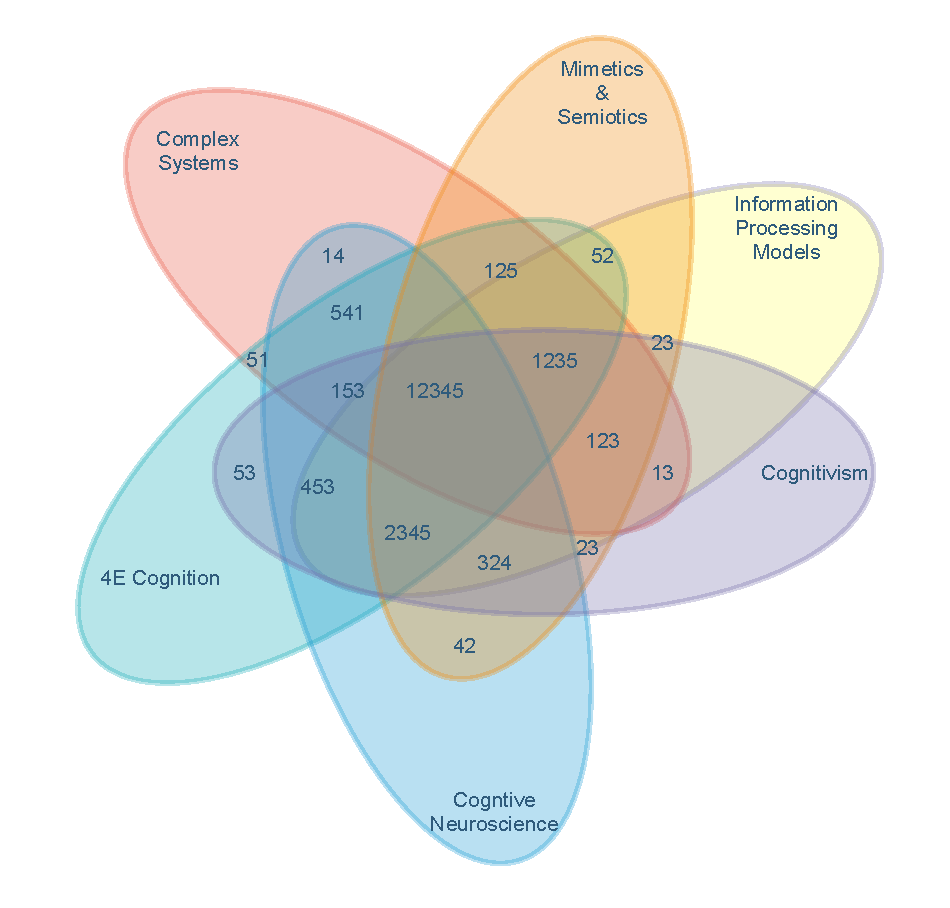
\includegraphics[width=75mm]{Roots Reconciliation Map.pdf}
\captionsetup{labelformat=empty} % makes sure dummy caption is blank
\caption{Reconciliation between multiple theoretical positions} % add dummy caption - otherwise \label won't work and figure numbering will not count up
\label{fig1} % use \ref{fig1} to reference to this figure
\end{figure} % avoid blank space here
\subsection{With cognitive-neuroscience}
The empirical findings of cognitive neuroscience cannot be disputed, because they are rigorously  conducted experiments. Their interpretation is valid, given their assumptions. Based on the model presented here we shall reinterpret their results, and motivate new experimental designs.  We do not agree brain as a coordinating point of action or a storehouse of memories, but enables them to store within the body and coordinate action by the body. We consider cognitive features as systemic properties of the entire LSMN, and of any localized part. 
\subsection{With generative grammar}
The core faculty of language is genetic (biologically granted) which evolved through organic evolution.  We agree with the view that human language develops from a predominant recursively generatable machine that can generate infinite combinations\cite{chomsky}.  We also consider that any theory that cannot account for this `fact' will not be considered worthy candidate.  We attempt to demostrate how the proposed model would ground generative grammar in the body reinforced by the social habits.
\subsection{With 4E-Cognition?}
Cognition is predominantly an action and takes time and effort to execute. Affordances of a cognitive agent provide meaning, and an inter-subjective space to share between agents. We also agree that much of human memories are externalized in multiple spaces outside the body. But we do not agree with the radical versions of 4E that human cognition can be explained without \textit{internal} representations. We have  memories \textit{stored} within the body that can be replayed.

One common argument that we often read in the literature on embodied cognition is that most of human cognition, including language, can be without \textit{internal} representations.\cite{linguistic_bodies}

\subsection{With Cognitive Robotics, AI and Machine Learning} 
Unlike the old-school AI, which is based on the model of an expert system (and a thorough information processing model), the recent breakthroughs in machine learning use neural networks. Cognitive robotics demonstrated that robots build a model of the environment with lesser dependence on internal databases. Data is built and used from the context (environment) while learning. These are more autonomous than any machines that were built in the past, indicating that this can be one of the confirming test-beds for cognitive theories. The model we propose is a synthesis of the idea that a layered mathematical computing machine can learn, and sensory sub-systems when mounted on proprioceptic motor components, which in turn are connected deferentially to the underlying computing network can develop habits in a habitat.  

\subsection{With Dynamical Systems}


\subsection{Novel Proposals}
\textbf{LSMN thesis}: The body is modeled as a sensory-motor-network. Nervous system provides layered network with the sensory-motor zones of the body. We do not model
the interaction schematic as brain-body-environment, with brain at the center. Instead it is body-environment, where the body is a layered network of sensory-motor sub-systems. 

The role of brain is to connect. By this, we are not undermining its role, but enhancing it. Connections can create emergent patterns, and connections can compute. Connected body can provide unitary experience. Connections can introduce delay in propagation, differential connections can generate variety. Cognition is an effect of the netework. 

Layered architecture creates an internal world, making reflexive actions possible. A part of the body can act with another part.  

\textbf{rHAPS thesis}: Motor control is obtained by haltability of motor action. This requires gaps in connections in an otherwise connected machine.  

The action patterns, which the SMN (the body) can’t afford to halt forming the inner layers of the network, are called beats. Beats are physiologically unaffordable for disengagement (e.g. heartbeats). The action patterns that can halt, generating variable patterns, are called haltable action patterns (HAPs) (e.g. breathing, walking, dancing, singing, talking etc). We argue that syntactic symbolic processing is impossible without variable haltability. Haltability is a ‘physiologically affordable anatomical disengagement’ (symbol ungrounding), which provides for a choice of actions. In our model, we argue that the genesis of syntax and freedom of choice are co-evolving features.
An orchestrated, variable, iterable and recursive set of action patterns become possible because of multiple zones of action patterns in the body (SMN). Here we argue that recursive action patterns make not only symbolic life possible but also tool use. Haltability itself provides recognisable reproducible variable experiences within an SMN generating meaning and memory. As an action-based ontological perspective, we not only support the view that the memory is for action (Glenberg), but also claim that reproducible action patterns ‘are’ memory, which is distributed in the SMN. 


\textbf{Computability thesis}: Only patterns can be computed. Patterns are relational configurations. By computing differentiation of differences we can obtain invariant results.  Similar or same results can be obtained from different inputs. This can be used as a logic of abstraction. 

(brought from the beats section) [Logically speaking, any data storage device requires a surface on which we can store (encode) the data. The surface can't be without a format. Analogically, the discs that we use in computers can't store data unless they are formatted using a file system. However, the file allocation table in a biological system emerges dynamically. Though we use this analogy to ascribe the role played by the beats in cognition, the differences between the architecture of a computing system that we are proposing is radically different from the von Newmann architecture.]





\section{Falsification criteria}
 Biological falsification criteria
 Cognitive Robotics based criteria: The robots themselves will be made in a layered manner. (Brooks kind of model, where there is no prior data, only of action patterns; behaviour is dependent on the environment, and data will be generated through interactions)
 
 \begin{itemize}
     \item We predict there is always some or other activity (eye saccades, dampened motor activity) while simulating, say like in forward models. This is a falsifiability criterion.
     \item
 \end{itemize}
 
%\clearpage
Topology contrast to be elaborated.

Recurrence is like rumination helping in assimilation and accommodation.

\section*{Acknowledgments}
We thank just about everybody.

\nolinenumbers

\bibliographystyle{Frontiers-Harvard}

\bibliography{test}

\end{document}


\section{Introduction}

For Original Research Articles \citep{conference}, Clinical Trial Articles \citep{article}, and Technology Reports \citep{patent}, the introduction should be succinct, with no subheadings \citep{book}. For Case Reports the Introduction should include symptoms at presentation \citep{chapter}, physical exams and lab results \citep{dataset}.



\section{Article types}

For requirements for a specific article type please refer to the Article Types on any Frontiers journal page. Please also refer to  \href{http://home.frontiersin.org/about/author-guidelines#Sections}{Author Guidelines} for further information on how to organize your manuscript in the required sections or their equivalents for your field

% For Original Research articles, please note that the Material and Methods section can be placed in any of the following ways: before Results, before Discussion or after Discussion.

\section{Manuscript Formatting}

\subsection{Heading Levels}

%There are 5 heading levels

\subsection{Level 2}
\subsubsection{Level 3}
\paragraph{Level 4}
\subparagraph{Level 5}

\subsection{Equations}
Equations should be inserted in editable format from the equation editor.

\begin{equation}
\sum x+ y =Z\label{eq:01}
\end{equation}

\subsection{Figures}
Frontiers requires figures to be submitted individually, in the same order as they are referred to in the manuscript. Figures will then be automatically embedded at the bottom of the submitted manuscript. Kindly ensure that each table and figure is mentioned in the text and in numerical order. Figures must be of sufficient resolution for publication \href{https://www.frontiersin.org/about/author-guidelines#ImageSizeRequirements}{see here for examples and minimum requirements}. Figures which are not according to the guidelines will cause substantial delay during the production process. Please see \href{https://www.frontiersin.org/about/author-guidelines#FigureRequirementsStyleGuidelines}{here} for full figure guidelines. Cite figures with subfigures as figure \ref{fig:Subfigure 1} and \ref{fig:Subfigure 2}.


\subsubsection{Permission to Reuse and Copyright}
Figures, tables, and images will be published under a Creative Commons CC-BY licence and permission must be obtained for use of copyrighted material from other sources (including re-published/adapted/modified/partial figures and images from the internet). It is the responsibility of the authors to acquire the licenses, to follow any citation instructions requested by third-party rights holders, and cover any supplementary charges.
%%Figures, tables, and images will be published under a Creative Commons CC-BY licence and permission must be obtained for use of copyrighted material from other sources (including re-published/adapted/modified/partial figures and images from the internet). It is the responsibility of the authors to acquire the licenses, to follow any citation instructions requested by third-party rights holders, and cover any supplementary charges.

\subsection{Tables}
Tables should be inserted at the end of the manuscript. Please build your table directly in LaTeX.Tables provided as jpeg/tiff files will not be accepted. Please note that very large tables (covering several pages) cannot be included in the final PDF for reasons of space. These tables will be published as \href{http://home.frontiersin.org/about/author-guidelines#SupplementaryMaterial}{Supplementary Material} on the online article page at the time of acceptance. The author will be notified during the typesetting of the final article if this is the case. 

\section{Nomenclature}

\subsection{Resource Identification Initiative}
To take part in the Resource Identification Initiative, please use the corresponding catalog number and RRID in your current manuscript. For more information about the project and for steps on how to search for an RRID, please click \href{http://www.frontiersin.org/files/pdf/letter_to_author.pdf}{here}.

\subsection{Life Science Identifiers}
Life Science Identifiers (LSIDs) for ZOOBANK registered names or nomenclatural acts should be listed in the manuscript before the keywords. For more information on LSIDs please see \href{https://www.frontiersin.org/about/author-guidelines#Nomenclature}{Inclusion of Zoological Nomenclature} section of the guidelines.


\section{Additional Requirements}

For additional requirements for specific article types and further information please refer to \href{http://www.frontiersin.org/about/AuthorGuidelines#AdditionalRequirements}{Author Guidelines}.

\section*{Conflict of Interest Statement}
%All financial, commercial or other relationships that might be perceived by the academic community as representing a potential conflict of interest must be disclosed. If no such relationship exists, authors will be asked to confirm the following statement: 

The authors declare that the research was conducted in the absence of any commercial or financial relationships that could be construed as a potential conflict of interest.

\section*{Author Contributions}

The Author Contributions section is mandatory for all articles, including articles by sole authors. If an appropriate statement is not provided on submission, a standard one will be inserted during the production process. The Author Contributions statement must describe the contributions of individual authors referred to by their initials and, in doing so, all authors agree to be accountable for the content of the work. Please see  \href{https://www.frontiersin.org/about/policies-and-publication-ethics#AuthorshipAuthorResponsibilities}{here} for full authorship criteria.

\section*{Funding}
Details of all funding sources should be provided, including grant numbers if applicable. Please ensure to add all necessary funding information, as after publication this is no longer possible.

\section*{Acknowledgments}
This is a short text to acknowledge the contributions of specific colleagues, institutions, or agencies that aided the efforts of the authors.

\section*{Supplemental Data}
 \href{http://home.frontiersin.org/about/author-guidelines#SupplementaryMaterial}{Supplementary Material} should be uploaded separately on submission, if there are Supplementary Figures, please include the caption in the same file as the figure. LaTeX Supplementary Material templates can be found in the Frontiers LaTeX folder.

\section*{Data Availability Statement}
The datasets [GENERATED/ANALYZED] for this study can be found in the [NAME OF REPOSITORY] [LINK].
% Please see the availability of data guidelines for more information, at https://www.frontiersin.org/about/author-guidelines#AvailabilityofData

\bibliographystyle{Frontiers-Harvard} %  Many Frontiers journals use the Harvard referencing system (Author-date), to find the style and resources for the journal you are submitting to: https://zendesk.frontiersin.org/hc/en-us/articles/360017860337-Frontiers-Reference-Styles-by-Journal. For Humanities and Social Sciences articles please include page numbers in the in-text citations 
%\bibliographystyle{Frontiers-Vancouver} % Many Frontiers journals use the numbered referencing system, to find the style and resources for the journal you are submitting to: https://zendesk.frontiersin.org/hc/en-us/articles/360017860337-Frontiers-Reference-Styles-by-Journal
\bibliography{test}

%%% Make sure to upload the bib file along with the tex file and PDF
%%% Please see the test.bib file for some examples of references

\section*{Figure captions}

%%% Please be aware that for original research articles we only permit a combined number of 15 figures and tables, one figure with multiple subfigures will count as only one figure.
%%% Use this if adding the figures directly in the mansucript, if so, please remember to also upload the files when submitting your article
%%% There is no need for adding the file termination, as long as you indicate where the file is saved. In the examples below the files (logo1.eps and logos.eps) are in the Frontiers LaTeX folder
%%% If using *.tif files convert them to .jpg or .png
%%%  NB logo1.eps is required in the path in order to correctly compile front page header %%%

\begin{figure}[h!]
\begin{center}
\includegraphics[width=10cm]{logo1}% This is a *.eps file
\end{center}
\caption{ Enter the caption for your figure here.  Repeat as  necessary for each of your figures}\label{fig:1}
\end{figure}

\setcounter{figure}{2}
\setcounter{subfigure}{0}
\begin{subfigure}
\setcounter{figure}{2}
\setcounter{subfigure}{0}
    \centering
    \begin{minipage}[b]{0.5\textwidth}
        \includegraphics[width=\linewidth]{logo1.eps}
        \caption{This is Subfigure 1.}
        \label{fig:Subfigure 1}
    \end{minipage}  
   
\setcounter{figure}{2}
\setcounter{subfigure}{1}
    \begin{minipage}[b]{0.5\textwidth}
        \includegraphics[width=\linewidth]{logo2.eps}
        \caption{This is Subfigure 2.}
        \label{fig:Subfigure 2}
    \end{minipage}

\setcounter{figure}{2}
\setcounter{subfigure}{-1}
    \caption{Enter the caption for your subfigure here. \textbf{(A)} This is the caption for Subfigure 1. \textbf{(B)} This is the caption for Subfigure 2.}
    \label{fig: subfigures}
\end{subfigure}

%%% If you don't add the figures in the LaTeX files, please upload them when submitting the article.
%%% Frontiers will add the figures at the end of the provisional pdf automatically
%%% The use of LaTeX coding to draw Diagrams/Figures/Structures should be avoided. They should be external callouts including graphics.

\end{document}

Cognition is a geometrical (GPS) processing problem. geometry of thought (\cite{Gardenfors2004-pi})

GPS needs a clock. Multiple signals, and a processor that maps the delay to distance. 

- which location the time has come
- we need multiple such locations where the time stamp comes
- 2nd law: greater the relative delay, greater the distance. 
- order of the world; patterns of the world; 
- HAPs are serial.
- HAPs give us naming the world
- arbitrary HAPs (disengaged) give us a arbitrary mapping; human languages.

- saturation and desaturation; 
- completely desaturated world is resolved only in terms of geometry
- saturated world comes in different shades; 



HAPS help the cognitive agent to generate relative geometry of the body.  


Sensory subsystem: signal generation, data production

motor subsystem: geometrical processing unit that constructs the space/world 

communication subsystem: multizonal connections and disconnections 


1 haps are grounded in faps. one fap zone 
2 there are multiple faps organized in antagonistic way
3 the antagonism is both mechanical and communication links

1. SMN resolves the relative location of the sensors/ transducers by self-modulation.

2. Self modulation changes the geometry of the SMN, the relative position of the sensors/transducers.

3. The resolution of internal and external world requires self-modulation and modulating the external world (which includes other self-modulating agents and inanimate world.)

4. The internal world is innate. Phylogeny and ontogeny provides the internal geometry.

5. External geometry (world) is created by using the principal of non-reflexive modulation. 

6. The major assumption of constructing a cognitive agent is that reflexivity is possible due to the network architecture of multiple sensory zones.

7. Another major assumption is that all the nodes of the network are in the same timezone.

8. Location of each sensor is resolved by applying the principle of the mapping between the delay and distance.

9. Modulation is change in distance between the sensors.

10. HAPs help in the modulation (9).

11. The change in network changes the geometry and modulation possibilities. Learning here is essentially change in geometry.

12. Newer forms of modulation (new HAPs) is learning. So, there is internal and external world are constructed by this process.

Movved from introduction section:

We do this by proposing a problem space where other models can be executed. The problem space is defined by postulating that the animate nature of cognitive agent's body is due to a \textit{muscular system}, whose role is to compute relative \textit{location} of phenomena (geometry), and a \textit{nervous system} whose role is to differentiate and integrate sensory data stream based on \textit{temporal} order (dynamics). In other words, it is a problem of constructing coordinates of a space-time and locating phenomena in that space-time. The cognitive body is a Geographical Positioning System (GPS) which has a clock relative to a timezone, and an algorithm to calculate the relative positions of the source of sensations. The source of sensations our model are both within the body as well as the external environment. Therefore, the problem-space is identified both in the body as well as at the body-environment interface. The multi-modal map resulting from this computation is the cognitive (phenomenological and epistemic) world. All cognition related problems shall be addressed in this space. 

Given this modified view of the body and its role in constructing the problem space, we attempt the reconciliation between cognitivism and enactivism. We agree with cognitivists that representations are at the core of cognition, and we also agree with enactivists that cognition is an enactive process. The problem-space described above can accommodate both actions and representations. We do this by stating that action \textit{patterns} are the units of cognitive processes, and not actions per se. And all action patterns are embodied. However, we present a distinct spectrum of multi-modal embodiment described in terms of degrees of saturation. The saturation reduces by progressively disengaging one modality from the other by modulation --- the process of abstraction. The action patterns \textit{appear} as disengaged and disembodied representations or concepts. Thus action patterns are real, while representations are nothing but manifestations of action patterns and their traces. In other words, perceptions and conceptions are located within the problem-space, which is resolved as a multi-dimensional spectrum of decreasing saturation. Therefore, philosophically, we meet Quine's challenge in 'The two dogmas of empiricism', naturalizing epistemology.


Research programs in cognitive science must address the established problems of symbol grounding, the frame problem, awareness, memory, subjectivity, the possibility of objective knowledge, generative grammar, mathematics, and various cultural practices. However, we cannot find them addressed in a single reductionist theory. However, a confluence of a finite set of coherent models supported by empirical and experimental evidence could address them. It is with this optimism we attempt to present this proposal.




